\documentclass[12pt]{article}

% BASIC PREAMBLE
/home/pedro/git/templates/preamble.tex

% THEOREM ENVIRONMENTS
% Theorems, propositions, etc (green)
\theoremstyle{darkgreentheorem}
\newtheorem{thm}{Theorem}
\newtheorem{lm}[thm]{Lemma}
\newtheorem{prop}[thm]{Proposition}
\newtheorem{cor}[thm]{Corollary}
\newtheorem{conj}[thm]{Conjecture}
% Definitions (blue)
\theoremstyle{darkbluedefinition}
\newtheorem{defn}[thm]{Definition}
% Examples (red)
\theoremstyle{darkredexample}
\newtheorem{exa}[thm]{Example}
% Remarks (black)
\theoremstyle{remark}
\newtheorem{rem}[thm]{Remark}
\newtheorem{pbl}[thm]{Problem}
\newtheorem{q}[thm]{Question}
\newtheorem{nota}[thm]{Notation}
\newtheorem{exe}[thm]{Exercise}

% MATH FONTS
% Mathbb
\newcommand{\N}{\mathbb{N}}
\newcommand{\Z}{\mathbb{Z}}
\newcommand{\Q}{\mathbb{Q}}
\newcommand{\R}{\mathbb{R}}
\newcommand{\1}{\mathbbm{1}}
\newcommand{\C}{\mathbb{C}}
\renewcommand{\P}{\mathbb{P}}
\newcommand{\CP}{\mathbb{CP}}
\newcommand{\bbE}{\mathbb{E}}
\newcommand{\bbT}{\mathbb{T}}
\newcommand{\bbD}{\mathbb{D}}
\newcommand{\cbbD}{\bar{\mathbb{D}}}
\newcommand{\Gm}{\mathbb{G}_{m}}
\newcommand{\bbA}{\mathbb{A}}
\newcommand{\V}{\mathbb{V}}
% Mathscr for categories
\newcommand{\scrC}{\mathscr{C}}
\newcommand{\Top}{\mathscr{T}op}
\newcommand{\CHaus}{\mathscr{CH}aus}
\newcommand{\ED}{\mathscr{ED}}
\newcommand{\A}{\mathscr{A}}
\newcommand{\CG}{\mathscr{CG}}
\newcommand{\Ab}{\mathscr{A}b}
\newcommand{\Set}{\mathscr{S}et}
\newcommand{\D}{\mathscr{D}}
\newcommand{\K}{\mathscr{K}}
\newcommand{\Db}{\mathscr{D}^{\mathrm{b}}}
\newcommand{\QCoh}{\mathscr{QC}oh}
\newcommand{\Coh}{\mathscr{C}oh}
% Mathcal for sheaves
\newcommand{\calA}{\mathcal{A}}
\newcommand{\calC}{\mathcal{C}}
\newcommand{\F}{\mathcal{F}}
\newcommand{\G}{\mathcal{G}}
\renewcommand{\L}{\mathcal{L}}
\newcommand{\M}{\mathcal{M}}
\renewcommand{\O}{\mathcal{O}}
\newcommand{\U}{\mathcal{U}}
\newcommand{\X}{\mathcal{X}}
\renewcommand{\H}{\mathcal{H}}
% Mathfrak for ideals
\newcommand{\m}{\mathfrak{m}}

% MATH OPERATORS
\DeclareMathOperator{\Hom}{Hom}
\DeclareMathOperator{\Ext}{Ext}
\DeclareMathOperator{\Fun}{Fun}
\DeclareMathOperator{\Cond}{Cond}
\DeclareMathOperator{\Ob}{Ob}
\DeclareMathOperator{\im}{im}
\DeclareMathOperator{\coker}{coker}
\DeclareMathOperator{\PSh}{PSh}
\DeclareMathOperator{\Sh}{Sh}
\let\Re\relax
\DeclareMathOperator{\Re}{Re}
\let\Im\relax
\DeclareMathOperator{\Im}{Im}
\DeclareMathOperator{\vol}{vol}
\DeclareMathOperator{\Supp}{Supp}
\DeclareMathOperator{\ihom}{\underline{Hom}}
\DeclareMathOperator{\iext}{\underline{Ext}}
\DeclareMathOperator{\GL}{GL}
\DeclareMathOperator{\Div}{Div}
\DeclareMathOperator{\Der}{Der}

% OTHER COMMANDS
\newcommand{\pe}{*_{proét}}
\renewcommand{\u}[1]{\underline{#1}}
\newcommand{\ot}{\otimes}
\newcommand{\op}{\oplus}
\newcommand{\fp}[1]{\times_{#1}}
\newcommand{\id}{\mathrm{id}}
\newcommand{\ev}{\mathrm{ev}}
\newcommand{\grd}{^{\bullet}}
\newcommand{\dual}{^{\vee}}
\newcommand{\db}{\marginnote{\dbend}}
\newcommand{\tms}{\times}
\newcommand{\sub}{\subseteq}
\newcommand{\epi}{\twoheadrightarrow}
\newcommand{\mono}{\hookrightarrow}
\newcommand{\LCA}{\mathrm{LCA}}

\title{Various lecture notes}
\author{Pedro Núñez}
\date{\today}

\begin{document}

\maketitle

\tableofcontents

\section{About these notes}

The purpose of these notes is to keep the material seen in lectures a bit organized and easily accesible from one single place, but they don't intend to be complete and they will surely be full of typos and mistakes\footnote{If you find any, please let me know! You can do this from GitHub or write me an email directly at pedro.nunez[at]math.uni-freiburg.de.}.

Warnings will be marked with a \href{https://en.wikipedia.org/wiki/Bourbaki_dangerous_bend_symbol}{dangerous bend} symbol on the margin \db.

\section{[CM] Talk 1 (Johan Commelin): Condensed Sets - 21.10.19}

\subsection{Introduction}

One of the main motivations for condensed mathematics is that topological algebraic objects have usually poor categorical and functorial properties.
For instance, topological abelian groups do not form an abelian category:

\begin{exa}
    $\R_{disc}\to \R$ is epi and mono, but not iso.
\end{exa}

Another motivation is coherent duality:

\begin{thm}
    Let $f\colon X\to Y$ be a proper or quasi-projective morphism of Noetherian schemes of finite Krull dimension. Then there exists a right adjoint $f^{!}$ to the derived direct image functor $f_{!}=Rf_{*}\colon \Db(\QCoh(X))\to \Db(\QCoh(Y))$.
\end{thm}

At some point analytic rings will come up.
We will then look at the category of solid modules, in which the 6-functor formalism works nicer than in the classical setting (e.g. when $f_{!}$ is not defined in the classical setting, $f_{!}$ takes non-discrete values in the condensed settings, which are "not there" in the classical setting).

\begin{defn}
    Pro\'{e}tale site of a point, denoted $\pe$, is the category of profinite sets with finite jointly surjective families of continuous maps as covers.
    A \textit{condensed set} (resp. group, ring, ...) is a sheaf of sets (resp. groups, rings, ...) on $\pe$.
    We denote by $\Cond(\scrC)$ the category of condensed objects of a category $\scrC$.
\end{defn}

\begin{defn}
    A \textit{condensed set} (resp. group, ring, ...) is a contravariant functor $X$ from $\pe$ to the category of sets (resp. groups, rings, ...) such that 
    \begin{enumerate}[label=\roman*)]
	\item $X(\varnothing)=*$.
	\item For all profinite sets $S_{1}$ and $S_{2}$ the natural map
	    \[ X(S_{1}\sqcup S_{2})\to X(S_{1})\times X(S_{2}) \]
	    is an isomorphism.
	\item For any surjection of profinite sets $f\colon S'\twoheadrightarrow S$ we get an induced\footnote{Since the pullback diagram is commutative, the image of $X(f)$ is indeed induces a morphism as claimed.} isomorphism
	    \[ X(S)\to \{ x\in X(S')\mid \pi_{1}^{*}(x)=\pi_{2}^{*}(x)\in X(S'\fp{S}S')\} \]
    \end{enumerate}
\end{defn}

We will call $X(*)$ the \textit{underlying object} in $\scrC$ of a condensed object.

\begin{rem}
    We will use $T$ for topological spaces vs. $X,Y$ for condensed sets, as opposed to Scholze's mixing of those notations.
\end{rem}

\subsection{Recollections on sheaves on sites}

Let $F$ be a presheaf on a site, which is just a contravariant functor to whatever category in which our sheaves are gonna take values.
If $U=\cup_{i}U_{i}$ is an open cover, the topological sheaf axiom could be phrased as: $F(U)$ is an equalizer of the diagram
\[ \prod_{i}F(u_{i})\rightrightarrows \prod_{i,j}F(U_{i}\cap U_{j}). \]
Note that $U_{i}\cap U_{j}$ is just the fiber product of the two inclusions.

\begin{defn}[Coverage]
    See definition 2.1 in \href{https://ncatlab.org/nlab/show/coverage}{nCat}.
\end{defn}

\begin{defn}
    $F$ a presheaf on $\scrC$.
    A collection $(s_{i})\in \prod_{i}F(U_{i})$ for $\{f_{i}\colon U_{i}\to U\}$ a covering is called a \textit{matching family} if for all $h\colon V\to U$ we have $g^{*}(s_{i})=h^{*}(s_{j})$ for $g$ and $h$ in the diagram
    \begin{center}
	\begin{tikzcd}
	    V\arrow{r}{h}\arrow{d}{g} & U_{j}\arrow{d}{f_{j}} \\
	    U_{i}\arrow{r}{f_{i}} & U
	\end{tikzcd}
    \end{center}
\end{defn}

\begin{defn}
    $F$ is a sheaf with respect to $\{U_{i}\to U\}$ if for all matching families $(s_{i})$ there exists a unique $s\in F(U)$ such that $f_{i}^{*}(s)=s_{i}$.
    We say that $F$ is a \textit{sheaf} if it is a sheaf for all covering families.
\end{defn}

\begin{rem}
    A sheaf of abelian groups is just a commutative group object in the category of sheaves of sets.
\end{rem}

\begin{thm}
    If $\scrC$ is a site, then $\Ab(\scrC)$ is an abelian category.
\end{thm}

\begin{defn}
    An additive category is a category in which the hom-sets are endowed with an abelian group structure in a way that makes composition bilinear and such that finite biproducts exist.
\end{defn}

Recall Grothendieck's axioms:
AB1) Every morphism has a kernel and a cokernel.
AB2) For every $f\colon A\to B$, the natural map $\operatorname{coim}(f)\to \im{f}$ is an iso.
AB3) All colimit exist.
AB4) AB3) + arbitrary direct sums are exact.
AB5) AB3) + arbitrary filtered colimits are exact.
AB6) AB3) + $J$ an index set, $\forall j\in J$ a filtered category (think of directed set) $I_{j}$, functors $M\colon I_{j}\to \scrC$, then
\[\varinjlim_{(i_{j}\in I_{j})_{j}}\prod_{j} M_{i_{j}}\to \prod_{j\in J}\varinjlim_{i_{j}\in I_{j}} M_{i_{j}} \]

\begin{thm}
    $\scrC$ a site. Then $\Ab(\scrC)$ satisfies AB3), AB4), AB5) and AB6).
\end{thm}

In fact, our case is even nicer:

\begin{thm}
    $\Cond(\Ab)$ in addition satisfies AB6) and AB4*).
\end{thm}

\subsection{Compactly generated topological spaces}

\begin{defn}
    A topological space $T$ is called \textit{compactly generated} if any function $f\colon T\to T'$ is continuous as soon as the composite $S\to T\to T'$ is continuous for all maps $S\to T$ where $S$ is compact and Hausdorff.
    See also \href{https://ncatlab.org/nlab/show/compactly+generated+topological+space}{nCat}.
\end{defn}

The inclusion functor $\CG \hookrightarrow \Top$ has a right adjoint $(-)^{cg}$.
If $T$ is any topological space, then the topology on $T^{cg}$ is the finest topology on $T$ such that $\sqcup_{S\to T}S\to T$ is continuous, where $S$ ranges over all compact Hausdorff spaces.

Let $T$ be a topological space.
We view $T$ as a presheaf on $\pe$ by setting $T(S)=\Hom_{\Top}(S,T)$ for all profinite sets $S$.
We denote this by $\u{T}$.
Claim: $\u{T}$ is a sheaf.
\begin{enumerate}[label=\roman*)]
    \item The first condition $\u{T}(\varnothing)=*$ is true, because there is exactly one morphism from the empty set to any topological space.
    \item $\u{T}(S_{1}\sqcup S_{2})=\u{T}(S_{1})\times \u{T}(S_{2})$ by universal property of disjoint union.
    \item For any surjection $S'\twoheadrightarrow S$ we get an isomorphism
	\[ \u{T}(S)\to \{ x\in \u{T}(S')\mid \pi_{1}^{*}(x)=\pi_{2}^{*}(x)\in \u{T}(S'\fp{S}S')\}\]
\end{enumerate}

Since $\Top\to \Cond(\Set)$ preserves products, group objects are preserved, so it maps topological groups to condensed groups etc.

\begin{prop}
    \begin{enumerate}[label=\roman*)]
	\item This functor is faithful and fully faithful when restricted to the full subcategory of compactly generated spaces.
	\item It admits a left adjoint $X\mapsto X(*)_{top}$ where $X(*)_{top}$ gets the quotient topology of $\sqcup_{S\to X}S\to X(*)$ as above.
	    The counit $I(*)_{top}\to T$ agrees with $T^{cg}\to T$.
    \end{enumerate}
\end{prop}

Coming back to our original example:

\begin{exa}
    $\mathbb{R}_{disc}\to \mathbb{R}$ can be seen in the condensed world as $\u{\mathbb{R}_{disc}}\to \u{\mathbb{R}}$, i.e. from locally constant functions to continuous functions.
    This is still a mono, but now it is not an epi.
    The cokernel $Q$ can be described as $Q(S)=\{ S\to \mathbb{R}\text{ continuous }\}/\{ S\to \mathbb{R}\text{ locally constant }\}$.
    Note in particular that the underlying set of $Q$ is just $*$, reflecting the fact that the cokernel was trivial in the classical setting.
\end{exa}

\section{[LT] Lecture 1 - 22.10.19}

\subsection{Introduction and overview of the course}

An \textit{algebraic variety} is the solution set of a family of polynomial equations in $\C^{n}$.
For example, if $f(x,y,z,t)=xy-tz$, then
\[ V(f)=\{(x,y,z,t)\in \C^{4}\mid xy-tz=0\} \]
is an algebraic variety in $\C^{4}$.
Another example would be the parabola $\{ y-x^{2}=0\}\subseteq \C^{2}$.

Let us focus on $V(f)$ and set $t=1$.
Then $X=V(f)\cap \{ t=1 \}=\{(x,y,z)\in \C^{3}\mid xy=z\}$ can be seen as a family of complex curves parametrized by the variable $z$.
For $z=0$, the complex curve $X_{0}$ has an \textit{ordinary double point} at the origin:

\begin{figure}[h]
    \centering
    \includegraphics[scale=.5]{odpfiber}
    \caption{Topological picture of our ODP.}
    \label{fig:odpfibre}
\end{figure}

Singularities arise naturally while studying the topology of algebraic varieties, and ODP's are a particularly nice kind of singularities.

For $z\neq 0$ we get an equation which looks like $xy=1$.
In this case we have the following picture:

\begin{figure}[h]
    \centering
    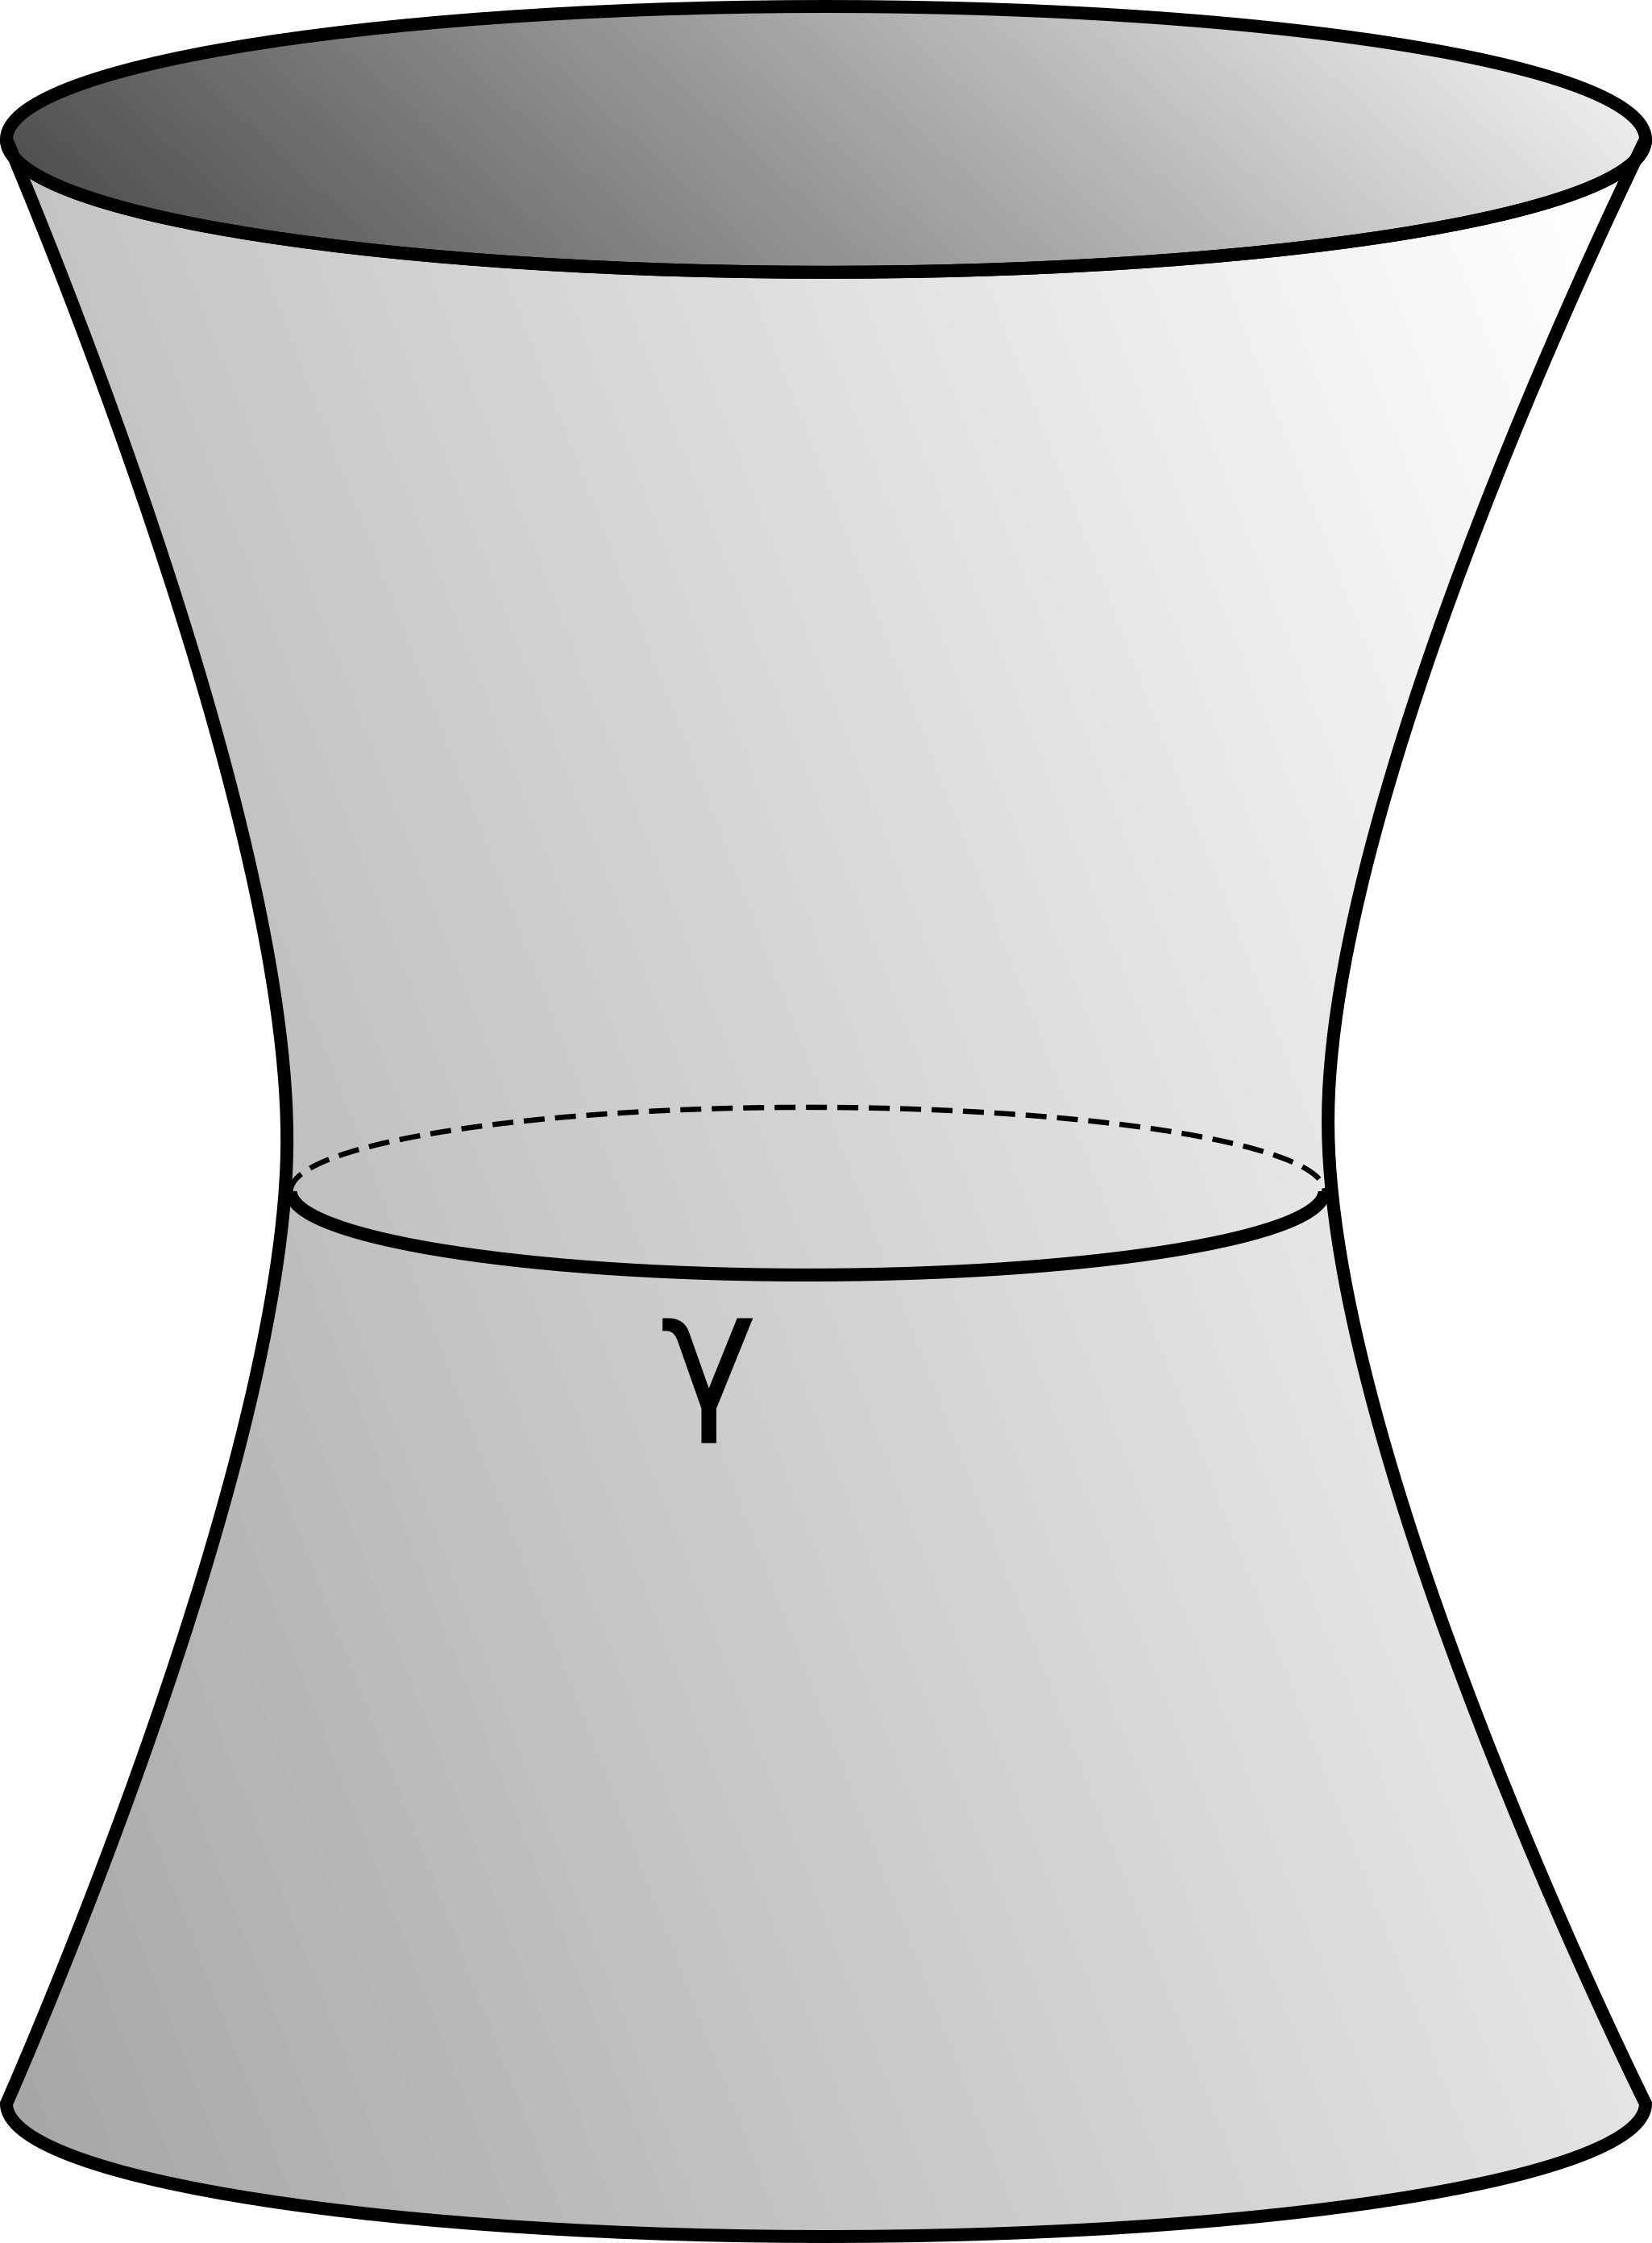
\includegraphics[scale=.8]{smoothfiber}
    \caption{Topological picture of $X_{z}$.}
    \label{fig:smoothfibre}
\end{figure}

As $z\to 0$, the central loop $\gamma$ contracts to the ordinary double point.
Note in particular that $X_{0}$ has trivial fundamental group (hence trivial $1$-homology), whereas $X_{z}$ does not.

We have a projection $\pi\colon X\to \C$, and Ehresmann's lemma tells us that for all disks $D\subseteq \C$ not containing $0$ we have $\pi^{-1}(D)\cong D\times X_{z_{0}}$ for any $z_{0}\in D$.

\begin{q}
    Given an arbitrary nonsingular algebraic variety $X\subseteq \C^{n}$, can we find a map $\pi\colon X\to \C$ such that the fibers $X_{t}$ are nonsingular for all but finitely many $t\in \C$ and such that the singular fibres have at worst ODP singularities?
\end{q}

Notice how we are missing information at infinity, e.g. $y=x^{2}$ versus $xy=1$.
The solution is to this is to replace $\C^{n}$ by $\CP^{n}$.

So let $X\subseteq\mathbb{P}^{n}$ be a nonsingular projective variety.
Then we have:

\begin{thm}
    There exists a family $(H_{t})_{t\in \CP^{1}}$ of hyperplanes in $\CP^{n}$ with $H_{[a,b]}=aH_{0}+bH_{\infty}$ such that
    \begin{enumerate}
	\item $X\subseteq \bigcup_{t\in \CP^{1}}H_{t}$.
	\item $X_{t}=X\cap H_{t}$ is nonsingular except for finitely many critical values of $t$.
	\item $X_{t}$ has ODP singularities for each critical value $t$.
    \end{enumerate}
\end{thm}

We call $(X_{t})_{t\in \CP^{1}}$ a \textit{Lefschetz pencil}.
We get a rational map $X\dashrightarrow \CP^{1}$ sending $x\mapsto t$ whenever $x\in X_{t}$.
If $x\in X_{t}\cap X_{t'}$ for $t\neq t'$, then $x\in H_{0}\cap H_{\infty}$, so this rational map is not well-defined along $X\cap H_{0}\cap H_{\infty}$.
Blowing-up this subvariety of $X$ we resolve the indeterminacy of the rational map and get a morphism $\tilde{X}\xrightarrow{\pi} \CP^{1}$ as we wanted.

As an application we obtain:

\begin{thm}[Lefschetz Hyperplane theorem]
    $X\subseteq Y\subseteq \CP^{N}$ nonsingular varieties with $X$ a hypersurface in the $n$-dimensional variety $Y$, then
    \[ H_{*}(X)\to H_{*}(Y) \]
    is an isomorphism for $*<n-1$ and a surjection for $*=n-1$.
\end{thm}

In particular, if $Y=\CP^{n}$, we have
\[ H_{*}(\CP^{n})=\begin{cases} \Z & \text{if } $*$ \text{ is even,} \\ 0 & \text{ otherwise.} \end{cases}\]
If $X\subseteq \CP^{n}$ is a nonsingular hypersurface, then its homology will be that of projective sapce on all degrees other than $n-1$.
Its $n-1$ homology will depend on the variety, e.g. the ODP (trivial $1$-homology) vs the ruled surface (with $\gamma$ non trivial on $1$-homology) from before.

\begin{exa}
    $X$ elliptic curve in $\CP^{2}$ given by $y^{2}=x(x-1)(x-\lambda)$ for $\lambda\neq 0$.
    Let $L=\CP^{1}\subseteq \CP^{2}$ and $P\in \CP^{1}\setminus (X\cup L)$.
    We get $X\xrightarrow{\pi}\CP^{1}$ by projecting from $P$ to $L$.
\end{exa}

\section{[WS] Kodaria 1 (Jin Li) - 23.10.19}

\subsection{Chow's theorem}

Let $G_{i}=G_{i}(z_{1},\ldots,z_{n})$ be homogeneous polynomials of degree $d_{i}$ for $i\in \{1,\ldots,k\}$.
Let $V=V(G_{1},\ldots,G_{k})=\{w\in \C^{n+1}\setminus \{0 \}\mid G_{i}(w)=0 \text{ for all }i\in \{1,\ldots,k\}\}\subseteq \CP^{n}$.
Assume $(\frac{\partial G_{i}}{\partial z_{j}}(w))_{i,j}$ is surjective at any $w\in V$.
By Euler's theorem on homogeneous functions we have
\[ \sum_{j=0}^{n}z_{j}\frac{\partial G_{i}}{\partial z_{j}}=d_{i}G_{i}(z_{0},\ldots,z_{n}). \]
If $\tilde{w}=(\tilde{z}_{0},\ldots,\tilde{z}_{n})\in V$, then
\[ \sum_{j=0}^{n}\tilde{z}_{j}\frac{\partial G_{i}}{\partial z_{j}}|_{\tilde{w}}=0\]
$V\cap U_{i}$ for any $i\in \{0,\ldots,n\}$, $U_{i}=\{[z_{0}:\ldots:z_{n}]\in \CP^{n}\mid z_{i}\neq 0\}$.

For $i=0$, consider the chart $(U_{0},\phi_{0})$ with $\phi_{0}\colon U_{0}\to \C^{n}$ given by $[z_{0},\ldots,z_{n}]\mapsto (\frac{z_{1}}{z_{0}},\ldots,\frac{z_{n}}{z_{0}})$.
The inverse has a lift given by $\tilde{\psi}\colon \C^{n}\to \C^{n+1}\setminus \{0\}$ given by $(w_{1},\ldots,w_{n})\mapsto (1,w_{1},\ldots,w_{n})$.
\begin{center}
    \begin{tikzcd}
	\C^{n}\arrow{d}{\tilde{\psi}}\arrow{dr}{G\circ \tilde{\psi_{0}}} & \\
	\CP^{n}\arrow{r}{G} & \C^{k}
    \end{tikzcd}
\end{center}
$V\cap U_{0}=G^{-1}(\{0\})$.

$G\circ \tilde{\psi_{0}}\colon (w_{1},\ldots,w_{n})\mapsto (G_{1}(1,w_{1},\ldots,w_{n}),\ldots,G_{k}(1,w_{1},\ldots,w_{n}))$.
\[ \frac{\partial (G_{i}\circ \tilde{\psi_{0}})}{\partial w_{j}} = \frac{\partial G_{i}}{\partial z_{l}}\frac{\partial(\tilde{\psi_{0}})^{l}}{\partial w_{j}}|_{(\tilde{w_{1}},\ldots,\tilde{w_{n}})} \]
Call the LHS $A_{1}$.
\begin{equation}
    \frac{\partial G_{i}}{\partial z_{l}}|_{\tilde{w}=(1,\tilde{w}_{1},\ldots,\tilde{w}_{n})}\begin{pmatrix} 1 \\ \tilde{w}_{1} \\ \vdots \\ \tilde{w}_{n} \end{pmatrix} = 0
\end{equation}
Note also that
\[\frac{\partial (\tilde{\psi_{0}})^{l}}{\partial w_{j}}=\begin{pmatrix} 0 & \ldots & 0 \\ 1 & \ldots & 0\\ \vdots & & \vdots \\ 0 & \ldots & 1 \end{pmatrix}.\]

Now
\[(\frac{\partial G_{i}}{\partial z_{l}})=(a_{il})=\begin{pmatrix} a_{10} & \ldots & a_{1n} \\ \vdots & & \vdots \\ a_{k0} & \ldots & a_{kn}\end{pmatrix}\]
\[A_{1}=\begin{pmatrix} a_{11} & \ldots & a_{1n} \\ \vdots & & \vdots \\ a_{k1} & \ldots & a_{kn} \end{pmatrix}\]
Since $A$ is surjective and 
\[A\begin{pmatrix} 1 \\ \tilde{w}_{1} \\ \vdots \\ \tilde{w}_{n}\end{pmatrix}=0,\]
hence $A_{1}$ is surjective.

\begin{thm}[Chow]
    Every analytic closed subvariety $V\subseteq \CP^{n}$ is the zero locus of finite number of homogeneous polynomials.
\end{thm}

For this we will use as a black box:

\begin{lm}[Remmert-Stein]
    Let $U\subseteq \C^{n}$ be a domain, $S$ be an analytic subvariety of $U$ of dimension $m$, and $W$ be an analytic subvariety of $U\setminus S$ such that $\dim_{p}W>m$ for all regular points $p\in W$.
    Then $\bar{W}$ is analytic.
\end{lm}

Now we can prove Chow's theorem.
Let $\pi\colon \C^{n+1}\setminus \{ 0\}\to \CP^{n}$ be the projection.
Then $\pi^{-1}(V)$ has dimension at least $1$ everywhere in $\C^{n+1}\setminus \{0 \}$.
Moreover, $\pi^{-1}(V)$ is a cone missing the origin, so its closure is just $\pi^{-1}(V)\cup \{0\}$.
Set $S=\{0\}$ and $W=\pi^{-1}(V)$. 
Then $V'=\bar{W}=\pi^{-1}(V)\cup \{0\}$ is an analytic variety of $\C^{n+1}$ by the Remmert-Stein theorem.
In particular, near $0$ we cam write
\[ V'_{0}=U_{\varepsilon}(0)\cap V'=V(g_{1},\ldots,g_{k})\]
with $g_{i}$ holomorphic on $U_{\varepsilon }(0)$.
In particular each $g_{i}$ is analytic, so we may write it as $g_{i}=\sum_{n=1}^{\infty} g_{i,n}$ where each $g_{i,n}$ is a homogeneous polynomial.
Then $g_{i}(tz)=\sum_{n=1}^{\infty}g_{i,n}(z)t^{n}$ for all $x\in \C^{n+1}$ and all $t\in \C$.
If $z\in V'$, then $tz\in V'$ for all $t$, because $V'$ is a cone.
So $g_{i}(tz)\equiv 0$ implies $g_{i,n}(z)=0$ for all $i\in \{1,\ldots,k\}$ and all $n\in \N_{>0}$.
Therefore $V_{0}'=V(\{g_{i,n}\})$.
By Noetherianity, finitely many $g_{i,n}$ suffice, so we can write $V_{0}=V(g^{(1)},\ldots, g^{(m)})$ for some $g^{(i)}\in \{g_{i,n}\}$.
Hence $V=V(g^{(1)},\ldots, g^{(m)})$ in $\CP^{n}$ and this finishes the proof.

\subsection{Sheaves}

For precise definitions and results in this subsection see Wikipedia, Stacks or nLab.

Definition of \textit{sheaf} (of abelian groups) on a topological space $X$, \textit{stalk} of a sheaf at a point $x\in X$, \textit{germs} of a sheaf at a point... Note the similarities in terminology with plants.

\begin{exa}
    Constant sheaves $\Z,\Q,\R,\C$.
    Sheaf of smooth functions $\calC^{\infty}$ and its units $\calC^{*}$.
    Sheaf of regular functions $\O$ and units $\O^{*}$.
    Sheaf of meromorphic functions $\M$ and $\M^{*}$.
\end{exa}

Maps between sheaves, their kernels and their cokernels.
Short exact sequences of sheaves.

\begin{exa}
    Let $M$ be a complex manifold.
    The sequence
    \[ 0\to \Z\to \O\xrightarrow{\exp} \O^{*}\to 0 \]
    is exact.
\end{exa}

Definition of \v{C}ech cohomology of a sheaf $\F\in \Sh(M)$ with respect to an open cover $\U$, which we denote by $H^{p}(\U,\F)$ on degree $p$, and \v{C}ech cohomology of the sheaf $F$ as their direct limit over refinements, denoted $\check{H}^{p}(M,\F)$.

\begin{thm}[Leray]
    If $\U$ is an acyclic cover, i.e. if there are no higher \v{C}ech cohomologies with espect to this cover, then the \v{C}ech complex associated to this cover computes \v{C}ech cohomology.
\end{thm}

Long exact sequence in \v{C}ech cohomology induced by a short exact sequence of sheaves.

\subsection{A bit of Hodge theory}

Decomposition of the tangent space at a point of a complex manifold, its tensor algebras, $\partial $ and $\bar{\partial }$ operators, Dolbeault cohomology groups, harmonic and Hodge decomposition.
See \cite{gh78} or \cite{voi07}.

\section{[LT] Lecture 2 - 24.10.19}

\begin{rem}
    Exercise sessions will be Thursday from 13h to 15h on SR318 (Starting next week).
\end{rem}

As pointed out last week, we want to look at polynomials and their solutions sets.
But polynomials are a bit too rigid.
Instead, we look at polynomials as truncated power series, or more generally as \textit{analytic functions}, which are functions which locally can be represented as power series.
We will see that these are the same as holomorphic functions.
In particular, every holomorphic function is $C^{\infty}$.
\begin{multline*}
    \text{polynomials} \Rightarrow \text{convergent power series} \Rightarrow \text{analytic} \Leftrightarrow \\
    \Leftrightarrow \text{holomorphic} \Rightarrow C^{\infty}\Rightarrow \text{continuous} \Rightarrow \text{abominations}
\end{multline*}

If we were analysts we would start at the bottom and then try to swim up.
Instead we will start from the top and float downstream.

\begin{nota}
    $\bbE=\R$ or $\C$.
    $z=(z_{1},\ldots,z_{n})\in \bbE^{n}$, $r\in \R_{\geqslant 0}$.
    Recall
    \[ |z|=\sqrt{2}{z_{1}\bar{z_{1}}+\cdots + z_{n}\bar{z_{n}}}, \]
    \[ \bbD(z,r)=\{w\in \bbE^{n}\mid |z-w|<r\}, \text{ and} \]
    \[ \cbbD(z,r)=\{ w\in \bbE^{n}\mid |z-w|\leqslant r\} \]
    called oepn and closed disks respectively.
    We call $\cbbD(z_{1},r_{1})\times \cdots \times \cbbD(z_{n},r_{n})$ an \textit{open polydisk}.
\end{nota}

\subsection{Formal power series}

\begin{defn}
    Let $a=(a_{1},\ldots,a_{n})\in \C^{n}$.
    A \textit{formal power series} centered at $a$ is an expression of the form
    \[ f(z)=f(z_{1},\ldots,z_{n})=\sum_{(r_{1},\ldots, r_{n})\in \Z^{n}_{\geqslant 0}}c_{r_{1}\cdots r_{n}}(z_{1}-a_{1})^{r_{1}}\cdots (z_{n}-a_{n})^{r_{n}} \]
    with $c_{r_{1},\ldots,r_{n}}\in \C$.
\end{defn}

\begin{rem}
    We will restrict our attention to absolutely convergent series, so we do not need to order the indices in the sum to discuss convergence.
\end{rem}

\begin{defn}
    The series above \textit{converges (uniformly) absolutely} on $X\subseteq \C^{n}$ if for all $z\in X$ the series of real numbers
    \[\sum_{(r_{1},\ldots,r_{n})} |c_{r_{1},\ldots,r_{n}}(z_{1}-a_{1})^{r_{1}}\cdots (z_{n}-a_{n})^{r_{n}}| \]
    converges (uniformly).
\end{defn}

Recall that $\sum_{n}c_{n}z^{n}$ converges absolutely on $\bbD(0,R)$ where $R=\frac{1}{\operatorname{limsup}_{n\to\infty}{|c_{n}|^{\frac{1}{n}}}}$.
It converges uniformly absolutely on each compact $K\subseteq \bbD(0,R)$.

\begin{exa}[Geometric series]
    The geometric series with ration $z=(z_{1},\ldots,z_{n})\in \C^{n}$ is defined as $\sum_{r_{1},\ldots,r_{n}}z_{1}^{r_{1}}\cdots z_{n}^{r_{n}}$.
    It converges (uniformly) absolutely on (compact subsets of) $\bbD(0,1)^{n}$ with sum equal
    \[ \prod_{k=1}^{n}\sum_{r_{k\geqslant 0}}z_{k}^{r_{k}}=\frac{1}{(1-z_{1})\cdots (1-z_{n})} \]
\end{exa}

\begin{lm}[Abel]
    Consider the series above, $w\in \C^{n}$ and $M\in \R_{>0}$.
    If $|c_{r}(w-a)^{r}|=|c_{r_{1},\ldots,r_{n}}(w_{1}-a_{1})^{r_{1}}\cdots (w_{n}-a_{n})^{r_{n}}<M$ for each $r\in \Z^{n}_{\geqslant 0}$, then $f(z)$ converges uniformly absolutely on each compact $K\subseteq D=\bbD(a_{1},\rho_{1})\times \bbD(a_{n},\rho_{n})$, where $\rho_{i}:=|w_{i}-a_{i}|$.
    \begin{proof}
	WLOG $\rho_{k}>0$ for all $k\in \{1,\ldots,n\}$ (otherwise we'd have $D=\varnothing$).
	Let $K\subseteq D$.
	Then let $\delta_{k}:=\max_{z\in K}\frac{|z_{k}-a_{k}|}{\rho_{k}}<1 $.
	Then for all $z\in K$ and for all $r\in \Z^{n}_{\geqslant 0}$ we have
	\[ |c_{r}(z-a)^{r}|\leqslant |c_{r}\rho^{r}|\leqslant M\delta^{r}.\]
	Since all $\delta_{k}<1$, by the previous example $\sum_{r}M\delta^{r}$ converges uniform absolutely on $K$.
    \end{proof}
\end{lm}

\begin{defn}
    Uniform absolute convergence on compacts is also called \textit{compact convergence}.
\end{defn}

\subsection{Analytic functions}

\begin{defn}
    Let $U\subseteq \C^{n}$ open.
    \begin{enumerate}[label=\roman*)]
	\item $f\colon U\to \C$ is \textit{analytic} at $a\in U$ if there exists an open neighbourhood $a\in V\subseteq U$ and $c_{r}$ such that $f(z)=\sum_{r}c_{r}(z-a)^{r}$ converges compactly on $V$.
	\item $f\colon U\to \C$ is \textit{analytic} on $U$ if it is analytic at each point of $U$.
	\item $f\colon U\to \C^{n}$ is \textit{analytic} on $U$ if each component $f_{k}$ is for all $k\in \{1,\ldots, n\}$.
    \end{enumerate}
\end{defn}

\begin{exe}
    Analytic at $a$ implies continuous at $a$.
\end{exe}

\begin{exe}
    If $f,g$ are analytic, then so are $f+g$, $f-g$ and $g\circ f$ where defined.
\end{exe}

\begin{exe}
    Let $U\subseteq C^{n}$ be an open subset, let $z\in U$ and $w\in \C^{n}$.
    Let $V=\{c\in \C\mid z+cw\in U\}\subseteq \C^{n}$.
    \begin{enumerate}[label=\roman*)]
	\item $V$ is open and $0\in V$.
	\item For all $f\colon U\to \C$ analytic we have that $g(t)=f(z+tw)$ is analytic on $V$.
    \end{enumerate}
\end{exe}

\begin{thm}[Identity theorem]
    If $\varnothing \neq V\subseteq U\subseteq \C^{n}$ are open with $U$ connected and $f\colon U\to \C$ is analytic with $f|_{V}=0$, then $f=0$.
    \begin{proof}
	If $f(z)\neq 0$ for some $z\in U$, then by continuity of $f$ we would have that $f$ is nowhere zero on some open nbhd of $z$.
	Let $Z=\{w\in U\mid f \text{ vanishes in an open nbhd of }w\}$.
	Then $Z$ is closed in $U$ by what we just said.
	Also, $V\subseteq Z$ as $V$ is open.
	Let $w\in Z$ and choose a polydisk $w\in D=\bbD(w_{1},r_{1})\times \cdots \times \bbD(w_{n},r_{n})\subseteq U$.
	If we show that $D\subseteq Z$, then every point of $Z$ is in its interior and $Z$ is therefore open.
	
	So let $z\in D$ with $z\neq w$.
	Consider now $W=\{c\in \C\mid w+c(z-w)in \U\}\subseteq \C$, which is open by the previous exercise\footnote{This step allows us to reduce our problem in several complex variables to a problem on a single complex variable.}, and $g\colon t\mapsto f(w+t(z-w))$ is analytic on $W$.
	The identity theorem for single-variable analytic functions implies that $g=0$ in a nbhd of $w$.
	Since $D$ is convex, $[0,1]\subseteq W$.
	By the identity theorem in one variable, $g=0$ on an open nbhd of $[0,1]$.
	Hence $g(1)=f(z)=0$, so $f$ vanishes on $D$ and $D\subseteq Z$.
    \end{proof}
\end{thm}

\subsection{Topology}

Definition of topological space and examples (cofinite topology, Zariski topology).
Continuous maps, homeomorphisms (isomorphism in the category of topological spaces).
Example: graph of $f\colon X\to Y$ defined as $\Gamma_{f}=X\fp{X}Y$ maps homeomorphically onto $X$ via the first projection.
Subspace topology.

Connectedness, example: unit interval.
Continuous image of connected is connected.

Hausdorffness, example: euclidean topology on $\R^{n}$.
Non-example: real line with two origins\footnote{These two examples show that Hausdorffness is not a local property, because the real line with two origins is locally the same as $\R$.}

Equivalently, $X$ is Hd if and only if $\Delta\subseteq X\times X$ is closed.
Hausdorffness is hereditary.

\section{[FS] Matthias Paulsen - The construction problem for Hodge numbers - 25.10.19}

In characteristic $0$ this is j.w. with Stefan Schreieder.
In positive characteristic this is j.w. with v. Dobbeen de Bruyn.

\subsection{Overview over complex numbers}

$X$ smooth projective variety.
Then we have Hodge theory, which allows us to decompose
\[ H^{k}(X,\C)=\bigoplus_{p+q=k}H^{p,q}(X), \]
where $H^{p,q}(X)\cong H^{q}(X,\Omega^{p})$.
The \textit{Hodge numbers} are $h^{p,q}(X)=\dim_{\C}H^{p,q}(X)$.
We usually arrange the Hodge numbers in the \textit{Hodge diamond}
\begin{center}
    \begin{tikzcd}
	& & & h^{n,n} & & & \\
	& & h^{n,n-1} & & h^{n-1,n} & & \\
	& & & \cdots & & & \\
	h^{n,0} & & & & & & h^{0,n} \\
	& & & \cdots & & & \\
	& & h^{1,0} & & h^{0,1} & & \\
	& & & h^{0,0} & & &
    \end{tikzcd}
\end{center}

\begin{exa}
    Let $X\subseteq \P^{4}$ be a hypersurface of degree $4$.
    Then its Hodge diamond is
    \begin{center}
	\begin{tikzcd}
	    & & & 1 & & & \\
	    & & 0 & & 0 & & \\
	    & 0 & & 1 & & 0 & \\
	    5 & & 30 & & 30 & & 5 \\
	    & 0 & & 1 & & 0 & \\
	    & & 0 & & 0 & & \\
	    & & & 1 & & & \\
	\end{tikzcd}
    \end{center}
\end{exa}

We know:
\begin{enumerate}[label=\roman*)]
    \item $h^{p,q}=h^{q,p}$.
    \item $h^{0,0}=1$.
    \item $h^{p,q}\geqslant h^{p-1,q-1}$ if $p+q \leqslant n$.
\end{enumerate}

\begin{q}
    Given $(h^{p,q})_{p,q}$ such that $i)$, $ii)$ and $iii)$ hold.
    Does there exist $X$ with $h^{p,q}(X)=h^{p,q}$ for all $p,q$?
\end{q}

\begin{itemize}
    \item [1989] Partial results in dimensions $2$ and $3$.
    \item [2013] Kotschick and Schreieder determined the Hodge ring of Kaehler manifolds and showed that there are no linear relations besides of the previous three.
    \item [2015] Schreieder.
	\subitem In any dimension $n$, a given row $k<n$ can be always achieved, except if $k=2p$, in which case we need $h^{p,p}\geqslant O(p)$.
	\subitem If we ignore the middle row, the outer Hodge numbers and the middle column, then everything else can be arbitraty.
	\subitem Negative results: the previous question has negative answer, e.g. in dimension three, if we assume that $h^{1,1}=1=$ and $h^{0,2}\geqslant 1$, then $h^{3,0}<12^{6}h^{2,1}$.
\end{itemize}

\begin{q}[Kollar]
    Are there any polynomial relations between the Hodge numbers, besides the ones induced by the symmetries above?
\end{q}

\begin{q}
    Besides the "unexpected" inequalities, are there also number theoretic restrictions?
\end{q}

\begin{itemize}
    \item [2019] Schreider and P.: modulo any integer $m\geqslant 1$, any Hodge diamond $(h^{p,q})_{p,q}$ satisfying the symmetries\footnote{Note that condition $iii)$ vanishes.} above is realizable by a smooth projective variety $X$, i.e. such that
	\[ h^{p,q}(X)\equiv h^{p,q} (\text{mod } m). \]
\end{itemize}

\begin{cor}
    There are no polynomial relations and there are no "number theoretic" restrictions.
\end{cor}

The proof can be devided into two parts corresponding to the outer Hodge numbers and the remaining ones.
The outer Hodge numbers are birational invariants.
The first part is to produce a variety which has the right outer Hodge numbers.
And then all the inner ones can be obtain by repeated blow-ups.
    
\subsection{Constructions}

We will have $3$ building blocks:
\begin{itemize}
    \item Products (and then use Kuenneth's formula).
    \item Hypersurfaces to reduce the dimension again (apply Lefschetz hyperplane theorem, picture [A]).
    \item Blow-ups of subvarieties (see picture [B]).
\end{itemize}

We start then with a curve, in which the problem is completely solvable:
\begin{center}
    \begin{tikzcd}
	& 1 & \\
	g & & g\\
	& 1 &
    \end{tikzcd}
\end{center}

Starting from this we can build up our Hodge diamonds modulo $m$.

\subsection{Positive characteristic}

We don't have complex conjugation, but we still have Serre duality imposing its 180 degrees rotation on the Hodge diamonds.
Is this the only restriction?

\begin{exa}[Serre]
    Construction of a surface with Hodge diamond
    \begin{center}
	\begin{tikzcd}
	    & & 1 & & \\
	    & 0 & & 1 & \\
	    ? & & ? & & ? \\
	    & 0 & & 1 & \\
	    & & 1 & & \\
	\end{tikzcd}
    \end{center}
\end{exa}

It seems that Matthias is up to something cool using this example!

\section{[CM] Talk 2 (Pedro Núñez) - Condensed Abelian Groups - 28.10.19}

See the full script on \href{https://github.com/pedro-nlb/cag}{GitHub}.

\subsection{Recollections from the previous talk}

Recall $\pe$ and $\A=\Sh(\pe,\Ab)$.

Equivalent description of $\A$ from last talk.

\subsection{A nicer description of our category}

\begin{defn}
    Extremally disconnected.
\end{defn}

Note that $\mathscr{ED}\subsetneq \mathscr{CH}$.

\textbf{Fact:} $S\in \mathscr{CH}$ is in $\mathscr{ED}$ if and only if every surjection $S'\twoheadrightarrow S$ from a compact Hausdorff space admits a section.
Using Stone-\v{C}ech compactification $\beta$, this implies that every $S\in \mathscr{CH}$ admits a surjection from an extremally disconnected set
\[ \exists \tilde{S}=\beta(S_{disc})\twoheadrightarrow S \]

\begin{lm}
    $\A=\Sh(\ED,\Ab)$.
\end{lm}

\begin{cor}
$\A=\{ \F\in \Fun(\ED^{op},\Ab)\mid i) \wedge ii)\}$.
\end{cor}

\begin{cor}
(Co)limits exist in $\A$ and can be constructed pointwise.
\end{cor}

\subsection{Abelianity and compact-projective generation}

Recall definition of Grothendieck category.

\begin{thm}
    $\A$ is abelian with (AB6) and (AB4*) and it is generated by compact projective objects.
\end{thm}

\begin{cor}
    $\A$ has enough injectives and projectives.
\end{cor}

\begin{center}
    \textbf{--- BREAK ---}
\end{center}

\subsection{Closed symmetric monoidal structure}

Briefly outline monoidal categories.

\begin{prop}
    $\A$ is symmetric monoidal and the functor $\Z[-]\colon \Cond(\Set)\to \A$ is symmetric monoidal.
\end{prop}

\begin{prop}
    For all condesned set $\X$, the condensed abelian group $\Z[\X]$ is flat, i.e. the functor $\Z[\X]\ot (-)$ is exact.
\end{prop}

\begin{prop}
    For all $\F\in\A$ the functor $\F\ot(-)$ has a right adjoint $[\F,-]$, i.e. $\A$ is closed symmetric monoidal.
\end{prop}

\subsection{Derived category}

Brief description.

\begin{rem}
    Triangulated structure and the problem it carries.
\end{rem}

Basic derived functors
\[ RF\colon \D^{+}(\A)=\K^{+}(\mathcal{I})\to \D(\mathscr{B}). \]

\begin{exa}
    $\Hom(-,\F)$ and $\Hom\grd(-,\F\grd)$.
\end{exa}

Extension to the whole $\D$ using Spaltenstein's resolutions.
Formula
\[ \Hom_{\D}(\F\grd,\G\grd[i])=\Ext^{i}(\F\grd,\G\grd).\]
Closed symmetric monoidal structure.

\begin{exa}
    $\Z[\X]\ot^{L}(-)=\Z[\X]\ot(-)$ is just degree-wise tensor product, because this functor is already exact so it need not be derived.
\end{exa}

\begin{prop}
    Compact generation.
\end{prop}

Mention Brown representability.

\section{[LT] Lecture 3 - 29.10.19}

\textbf{Goals for today:}
\begin{itemize}
    \item \textbf{Prop:} $f$ analytic $\Rightarrow f$ complex differentiable (holomorphic).
    \item \textbf{Cor:} $f$ analytic $\Rightarrow f\in \calC^{\infty}$.
    \item Implicit and inverse function theorems for analytic functions.
\end{itemize}

\subsection{Complex differentiable functions}

Recall: $U\subseteq \R^{n}$ open, $f\colon U\to \R^{m}$ is \textit{differentiable} at $a\in U$ if $\exists \R$-linear map $df_{a}\colon \R^{n}\to \R^{m}$ such that
\[ \lim_{h\to 0}\frac{f(a+h)-f(a)-df_{a}(h)}{|h|}=0.\]
With respect to the standard bases, $df_{a}$ is given by the \textit{Jacobian} matrix $J_{f}(a)=(\frac{\partial f_{i}}{\partial f_{j}})_{i,j}$.

We say that $f\colon U\to \R^{m}$ is $\calC^{\infty}$ or \textit{smooth} if all partial derivatives exist (to all orders) and are continuous.

Recall also that $f\in \calC^{1}$ implies $f$ differentiable.

\begin{defn}
    $X\subseteq \R^{n}$ not necessarily open, $f\colon X\to \R^{m}$ is \textit{differentiable} or $\calC^{\infty}$ if for all $x\in X$ we can find an open nbhd $x\in U\subseteq \R^{n}$ and a differentiable or $\calC^{\infty}$ function $F\colon U\to \R^{m}$ such that $F|_{X\cap U}=f|_{X\cap U}$.
\end{defn}

\begin{defn}
    Let $U\subseteq \C^{n}$ open.
    We say that $f\colon U\to \C$ is \textit{complex differentiable} at $a\in U$ if it is continous and
    \begin{enumerate}[label=\roman*)]
	\item if $n=1$, then the limit $f'(a):=\lim_{z\to a}\frac{f(z)-f(a)}{z-a}$ exists.
	\item if $n>1$, then for all $1\leqslant k\leqslant n$ and for all $z_{1},\ldots,\hat{z_{k}},\ldots,z_{n}$ the function
	    \[ f_{k}(z):=f(z_{1},\ldots,z_{k-1},z,z_{k+1},\ldots,z_{n})\]
	    is complex differentiable as in $1)$.
    \end{enumerate}
\end{defn}

\begin{exa}
    $\Re,\Im\colon \C\to \R$ are $\calC^{\infty}$, not complex differentiable.
\end{exa}

If $f$ is complex differentiable, then $\frac{\partial f}{\partial x_{i}},\frac{\partial f}{\partial y_{i}}$ exist and are continuous, i.e. $f\in \calC^{1}$.

\begin{prop}
    Let $U\subseteq \C^{n}$ open and $f\colon U\to \C$ is analytic.
    Then $f$ is complex differentiable and $f'$ is analytic.
    \begin{proof}
	$f(z_{1},\ldots,z_{n})=\sum_{r}c_{r}(z-a)^{r}$ locally near $a\in U$.
	Continuity is OK, we need to show that
	\[ \sum c_{r}(\zeta_{1}-a_{1})^{r_{1}}\cdots (\zeta_{n-1}-a_{n-1})^{r_{n-1}}(z_{n}-a_{n})^{r_{n}}\]
	is complex differentiable for all $(\zeta_{1},\ldots,\zeta_{n})$ with respect to $z_{n}$.
	This is a power series in a single variable, hence complex differentiable.
    \end{proof}
\end{prop}

\begin{cor}
    $f$ analytic implies $f$ smooth.
    \begin{proof}
	$f$ analytic implies $f'$ analytic, hence $f''$ analytic, and so on.
    \end{proof}
\end{cor}

\subsection{Implicit function theorem}

\begin{nota}
    We denote by $\C[[z_{1},\ldots,z_{n}]]$ the ring of formal power series in $z_{1},\ldots,z_{n}$ centered at $0$ (with Cauchy product as multiplication) and by $\C\{z_{1},\ldots,z_{n}\}$ the subring of all power series convergent in a nbd of $0$.
\end{nota}

\begin{lm}\footnote{Typical proof with power series: do the naive thing inducting on the degree and the number of variables.}
    Let $f(z_{0},\ldots,z_{n})=\sum_{r} c_{r}z^{r}$ with $c_{0,\ldots, 0}\neq 0$.
    Then $\exists !g\in \C[[z_{1},\ldots,z_{n}]]$ such that $fg=1$.
    \begin{proof}
	WLOG $c_{0,\ldots, 0}=1$.
	Let $z=(z_{1},\ldots,z_{n-1})$ and $w=z_{n}$.
	Let $f=\sum_{k}a_{k}(z)w^{k}$ with $a_{k}(z)\in \C[[z]]$.
	Let $g=\sum_{k} b_{k}(z)w^{k}$ with $b_{k}(z)\in \C[[z]]$.
	Then $fg=\sum_{l=0}^{\infty}(\sum_{k=0}^{l}a_{k}b_{l-k})w^{l}$.
	Call $\delta_{0,l}=\sum_{k=0}^{l}a_{k}b_{l-k}$.
	$l=0$ implies $1=a_{0}b_{0}$, hence $b_{0}=a_{0}^{-1}$.
	For $l>0$ we get $0=\sum_{k=0}^{l}a_{k}b_{l-k}a_{k}b_{l-k}$, hence
	\[b_{l}=-a_{0}^{-1}\sum_{k=1}^{l}a_{k}b_{l-k}.\]
    \end{proof}
\end{lm}

\begin{thm}[Formal implicit function theorem]\footnote{Near $0$ we have $f(z,w)=0$ iff $0=u(z,w)f(z,w)$ iff $0=w-r(z)$, i.e. the vanishing locus of $f$ is the graph of $r$ near $0$, hence this is indeed an implicit function theorem.}
    If $f\in \C[[z,w]]$, $f(0)=0$ and $\frac{\partial f}{\partial w}\neq 0$, then $\exists ! u\in \C[[z,w]]$ and $\exists ! r\in \C[[z]]$ such that $uf=w-r$ and $u(0)\neq 0$.
    \begin{proof}
	\begin{enumerate}[label=\arabic*)]
	    \item Consider the $\C$-linear maps
		\begin{align*}
		    R\colon \C[[z,w]] & \to \C[[z]] \\
		    p=\sum_{r}c_{r}(z)w^{r} & \mapsto c_{0}(z)
		\end{align*}
		\begin{align*}
		    H\colon \C[[z,w]] &\to \C[[z,w]] \\
		    p=\sum_{r}c_{r}w^{r} & \mapsto \frac{p-R(p)}{w}=\sum_{r>0}c_{r}w^{r-1}
		\end{align*}
	    \item $\forall p$ we have $p=wH(p)+R(p)$.
	    \item $H(f)$ is a unit by the previous lemma and $\frac{\partial f}{\partial w}\neq 0$.
	    \item Suffices to find $u$ s.t.
		\[ 0=H(w-uf)=H(w)-H(uf)\]
		\[ 0=1-H(uf) \quad (*) \]
		Indeed, $(*)$ and $2)$ imply that $R(w-uf)=w-uf$, hence $r:=w-uf\in \C[[z]]$ ($w=uf+(w-uf)=uf+r$).
	    \item \begin{multline*}
		    uf\overset{2)}{=} u(wH(f)+R(f))\\
		    =uwH(f)+uR(f)\\
		    (*)\Leftrightarrow 0=1-H(uf)\\
		    0=1-H(uwH(f)+uR(f)) \\
		    0=1-(\frac{uwH(f)-R(uwH(f))}{w})-H(uR(f)) \\
		    (**) 0=1-uH(f)-H(uR(f))
	    \end{multline*}
	\item $H(f)$ unit $\Rightarrow $ suffices to find $v=uH(f)$.
	    $\mu:=-R(f)H(f)^{-1}$ s.t. $u=vH(f)^{-1}$ satisfies $(**)$.
	\item \begin{multline*}
		(**)\Leftrightarrow 0=1-v+H(\frac{-uR(f)}{H(f)}H(f)) \\
		(***) 0=1-v+H(\mu v)
	    \end{multline*}
	\item $M\colon \C[[z,w]]\to \C[[z,w]]$ defined as $p\mapsto H(\mu p)$.
	    Note: if $z^{k}$ divides $p$, then $z^{k+1}$ divides $M(p)$.
	\item \begin{multline*}
		0=1-v+M(v) \\
		(***') v=1+M(v)
	    \end{multline*}
		$\C$-linearity of $M$ implies that $v=1+M(v)=1+M(1+M(v))$.
		Hence for all $k\geqslant 0$ we have
		\[ v=1+M(1)+\cdots +M^{k}(1)+M^{k}(v). \]
	\item $z^{k}$ divides $M^{k}(1)$, $z^{k+1}$ divides $M^{k+1}(v)$.
	    Hence $\sum_{k}M^{k}(1)$ is convergent as a formal power series.
	\item If $v$ satisfying $(***')$, then $v=\sum_{k}M^{k}(1)$.
	    Hence $v$ is unique and thus so are $u, r$.
	\item $v=\sum_{k}M^{k}(1)$ satisfies $(***')$.
	    $v=1+M(1)+\cdots +M^{k}(1)+W_{k}$, hence $z^{k+!}$ divides $W_{k}$ by $10)$.
		$v-1-M(v)=1+M(1)+\cdots +M^{k}(1)+W_{k}-1-M(1)-\cdots -M^{k}(1)-M^{k+1}(1)-M(W_{k})$, hence for all $k$ we have that $z^{k+1}$ divides $v-1-M(v)$.
		Therefore $v-1-M(v)=0$.
	\end{enumerate}
    \end{proof}
\end{thm}

\begin{thm}[Convergent implicit function theorem]
    With notation as above, if $f\in \C\{z,w\}$, then $u\in \C\{z,w\}$ and $r\in \C\{z\}$.
    \begin{proof}
	See Samuel-Zariski.
    \end{proof}
\end{thm}

\begin{exe}
    Formulate and deduce the analytic inverse and implicit function theorem.
\end{exe}

\subsection{More basic topology}

Product spaces: definition and universal property.
Example: $\R^{n}\cong \R\times \R^{n-1}$ with the usual topology.
Non example: $\C^{n+m}\not\cong \C^{n}\times \C^{m}$ with the Zariski topology.

Quotient spaces: definition and universal property.
Examples: $S^{1}=[0,1]/1\sim =\R/\Z$ and $\mathbb{T}^{2}$ gluing the boundary of the square $[0,1]^{2}$ appropriately.

Quasi-compactness: definition.
Non-example: $\R$.
Example: $[a,b]\subseteq \R$.
In $\R^{n}$ quasi-compact iff closed bounded.
More facts: union of qc is qc, continuous image of qc is qc, closed subset of qc is qc.

\section{[WS] Kodaira 2 (Vera) - Introduction to Hodge Manifolds - 30.10.19}

Outline for today:
\begin{enumerate}[label=\arabic*)]
    \item Recollections.
    \item Hodge Manifolds.
    \item Outlook: Kodaira's Embedding Theorem.
\end{enumerate}

\subsection{Recollections}

\subsubsection{Cohomology Theories}

1. Recall the \textit{Dolbeault-Cohomology} defined as
\[ H^{p,q}(X):=\frac{\ker(\bar{\partial}\colon \A^{p,q}(X)\to \A^{p,q+1}(X))}{\im(\bar{\partial}\colon \A^{p,q-1}(X)\to \A^{p,q}(X))}.\]

2. Recall the \textit{de Rham cohomology} defined as
\[ H_{dR}^{k}(X,\C)=\frac{\ker(d\colon \A_{\C}^{k}(X)\to \A_{\C}^{k+1}(X))}{\im(d\colon \A_{\C}^{k-1}(X)\to \A_{\C}^{k}(X))}, \]
where $\A_{\C}^{k}=\Gamma(X,\Lambda^{k}TX^{*}\ot \C)$.

\begin{thm}
    On a compact Kaehler manifold $(X,I,<\cdot,\cdot>)$ we have
    \[ H_{dR}^{k}(X,\C)\cong \bigoplus_{p+q=k}H^{p,q}(X).\]
\end{thm}

On the other hand, we have

\begin{thm}[de Rham Theorem]
    \[ H_{dR}^{k}(X,\C)\cong H^{k}(X,\C).\]
\end{thm}

3. Integral cohomology.

\begin{defn}
    Let $X$ be a compact complex manifold.
    A closed differential form $\varphi$ on $X$ is called \textit{integral} if its cohomology class $[\varphi]\in H^{k}_{dR}(X,\C)$ is in the image of the mapping
    \[ H^{k}(X,\Z)\to H^{k}(X,\C)\cong H_{dR}^{k}(X,\C). \]
\end{defn}

Today we will be interested in integral $(1,1)$-classes, i.e.
\begin{center}
    \begin{tikzcd}
	& H^{2}(X,\Z)\arrow[swap]{dl}{j_{*}}\arrow{d} \\
	H^{1,1}(X)\subseteq H_{dR}^{2}(X,\C)\arrow{r}{\cong} & H^{2}(X,\C)
    \end{tikzcd}
\end{center}
We denote $\tilde{H}_{dR}^{2}(X,\Z):= j_{*}H^{2}(X,\Z)$.

\subsubsection{Holomorphic line bundles and first Chern class}

Recall the exponential sequence
\[ 0\to \Z\to \O\xrightarrow{\exp}\O^{\times}\to 0\]
of sheaves.
Last week we have seen that this sequence is exact and thus it induces a long exact sequence of cohomology groups
\[ \cdots \to \check{H}^{1}(X,\O^{\times})\xrightarrow{\delta} \check{H}^{2}(X,\Z)\to \cdots \]

\textbf{Fact 1:} $\check{H}^{1}(X,\O^{\times})$ classifies holomorphic line bundles up to holomorphic isomorphism.

\textbf{Fact 2:} In the sequence above, $\delta$ is ``almost'' $c_{1}$.
\begin{center}
    \begin{tikzcd}
	H^{1}(X,\O^{\times})\arrow{r}{\delta}\arrow{dr}{c_{1}} & H^{2}(X,\Z)\arrow{d} \\
	& H_{dR}^{2}(X,\R)
    \end{tikzcd}
\end{center}
i.e. holomorphic line bundles have ``integral Chern classes''.

\begin{rem}
    Indeed, the Lefschetz $(1,1)$-theorem states that on compact Kaehler manifolds $X$ we have
    \[ c_{1}(H^{1}(X,\O^{\times}))=\tilde{H}^{2}(X,\Z)\cap H^{1,1}(X). \]
\end{rem}

In the proof of the previous commutative diagram, an explicit formula for the $(1,1)$-form representing $c_{1}(E,h)$, namely
\[ \frac{1}{2\pi i}\partial \bar{\partial} \log(h_{\alpha}),\]
where $h_{\alpha}$ is the metric on $U_{\alpha}$.

\subsubsection{Kaehler manifolds}

\begin{defn}
    Given a complex manifold $(M,I,g)$ where the complex structure $I$ is compatible with the metric $g$, we associate a $(1,1)$-form
    \[ w(\cdot,\cdot)=g(I\cdot,\cdot) \]
    called the \textit{Kaehler form}.

    We say that $M$ is Kaehler, if it admits some metric such that the associated Kaehler form is closed ($dw=0$).

    In that case, $w\in \A^{1,1}(M)$ defines a cohomology class $[w]\in H^{1,1}(M)$, called the \textit{Kaehler class}.
\end{defn}

\begin{exa}[The Fubini-Study metric on $\CP^{n}$]
    In homogeneous coordinates, the corresponding Kaehler form is given as
    \[ w_{a}=i\partial \bar{\partial}\log(|\zeta_{a}|^{2}+1) \]
    on $U_{a}=\{(z^{0}:\ldots:z^{n})\mid z^{a}\neq 0\}$.
    The map $\zeta_{a}\colon U_{a}\to \C^{n}$ sends $(z^{0}:\ldots:z^{n})\mapsto (\frac{z^{0}}{z^{a}},\ldots,\hat{1},\ldots,\frac{z^{n}}{z^{a}})$.
\end{exa}

From this we can also deduce the same for any projective complex manifold using the following:

\begin{lm}
    Let $(X,I,g)$ be a Kaehler manifold with Kaehler form $w$ and let $M$ be a complex submanifold.
    Then $g$ induces a Kaehler manifold on $M$, thus $M$ is a Kaehler manifold.
\end{lm}

\subsection{Hodge Manifolds}

\begin{defn}
    Let $(X,h)$ be a Kaehler manifold with Kaehler metric $h$ and let $w$ be the associated Kaehler form.
    If $w$ is integral, it is called a \textit{Hodge form} on $X$ and $h$ is called a \textit{Hodge metric}.
    A Kaehler manifold is called \textit{Hodge manifold} if it admits a Hodge metric.
\end{defn}

\begin{exa}[Complex projective space]
    Let $\CP^{n}$ be endowed with the Fubini-Study metric $g_{FS}$ and the associated Kaehler form $w_{FS}$.
    Then $w_{FS}$ is a Hodge form.
    Indeed, let $E\to \CP^{n}$ be the tautological line bundle.
    By Fact 2, $c_{1}(E)\in \tilde{H}^{2}(X,\Z)$.
    And we have
    \[ \left[\frac{1}{2\pi} w_{FS}\right] =-c_{1}(E).\]
    Thus $\CP^{n}$ is a Hodge manifold.
\end{exa}

\begin{exa}[Projective complex manifolds]
    Let $X$ be a projective complex manifold, i.e. $X\subseteq \CP^{n}$ as closed complex submanifold.
    The restriction of the Hodge form on $\CP^{n}$ is a Hodge form on $X$.
\end{exa}

\textbf{Fundamental fact:} all projective complex manifolds are Hodge.

\begin{exa}[Compact connected Riemann surfaces]
    Let $X$ be a compact connected Riemann surface.
    The claim is that $X$ is a Hodge manifold.
    We have $H^{2}(X,\C)\cong H_{0}(X,\C)\cong \C$.
    Moreover, $H^{2}(X,\C)\cong H^{1,1}(\C)$.
    Let $\tilde{w}$ be the Kaehler form associated to some metric on $X$.
    Then $[\tilde{w}]\in H^{1,1}(\C)$ generates $H_{dR}^{2}(X,\C)$.
    Let $c:=\int_{X}\tilde{w}$.
    Then $w:=\frac{1}{c}\tilde{w}$ is an integral positive form on $X$ of type $(1,1)$.
\end{exa}

\subsection{Outlook}

We will soon prove the converse of our fundamental fact, namely:

\begin{thm}[Kodaira's Embedding]
    Every Hodge manifold admits a closed immersion into $\CP^{n}$ for $n$ sufficiently large.
\end{thm}

Combining this with Chow's theorem seen last time, we obtain as a corollary that Hodge manifolds are always algebraic.

\section{[LT] Lecture 4 - 31.10.19}

\subsection{Key theorems}

\begin{thm}[Liouville]
    $f\colon \C^{n}\to \C$ bounded.
    Then $f$ constant.
    \begin{proof}
	Let $z,w\in \C^{n}$.
	We claim that $f(z)=f(w)$.
	Consider $h\colon c\mapsto z+c(w-z)$ from $\C\to \C^{n}$.
	This is analytic.
	Hence $g:=f\circ h$ is analytic.
	$\im(g)\subseteq \im(f)$, so $g$ is also bounded.
	By the $1$-dimensional Liouville theorem, $g$ is constant.
	But then $f(z)=g(0)=g(1)=f(w)$.
    \end{proof}
\end{thm}

\begin{thm}[Maximum modulus principle]
    $U\subseteq \C^{n}$ open connected, $f\colon U\to \C$ analytic, $a\in U$.
    If $|f(a)|\geqslant |f(z)|$ for each $z$ in an open nbd $a\in V\subseteq U$, then $f$ is constant on $U$.
    \begin{proof}
	Identity theorem implies that if $f$ is constant on $V$, then $f$ is constant on $U$.
	So WLOG $V=D$ a polydisk centered at $a$.
	Consider $z_{1}\mapsto f(z_{1},a_{2},\ldots,a_{n})$ from $D(a,r)$ to $\C$.
	This is analytic and its modulus attains a maximum at $z_{1}=a_{1}$.
	By the single variable maximum modulus principle, this map is constant on $D(a_{1},r_{1})$.
	
	Suppose $(z_{1},\ldots,z_{k})\mapsto f(z_{1},\ldots,z_{k},a_{k+1},\ldots,a_{n})$ is constant on $D(a_{1},r_{!})\times \cdots \times D(a_{k},r_{k})$ for some $1\leqslant k<n$.
	Then $\forall (w_{1},\ldots, w_{k},z_{k+1},a_{k+2},\ldots,a_{n})$, $z_{k+1}\mapsto f(w_{1},\ldots,w_{k},z_{k+1},a_{k+2},\ldots,a_{n})$ is analytic, its modulus has a maximum at $z_{k+1}=a_{k+1}$.
	This implies by the single variable case that it is constant.
	By induction, we win.
    \end{proof}
\end{thm}

\begin{thm}[Open mapping theorem]
    $U\subseteq \C^{n}$ connected open, $f\colon U\to \C$ nonconstant, analytic.
    If $V\subseteq U$ is open, then $f(V)\subseteq \C$ is open as well.
    \begin{proof}
	Let $z\in V$ and $w=f(z)$.
	It suffices to construct an open nbd of $w$ contained in $f(V)$.
	There exists an open polydisk $D$ centered at $z$ containedin $V$, and $V$ is a union of such polydisks.
	Hence WLOG $V=D$.

	$f$ nonconstant implies that $\exists z'\in D$ with $f(z)\neq f(z')$.
	The set $W=\{c\in \C\mid z+c(z'-z)\in D\}\subseteq \C $ is open.
	The composite $f\circ h\colon W\to \C$ is analytic and nonconstant.
	By the single variable open mapping theorem, $f\circ h$ is open.
	Hence $\im(f\circ h)\subseteq \C$ is open, and $\im(f\circ h)\subseteq f(V)$.
    \end{proof}
\end{thm}

\subsection{Cauchy-Riemann equations}

\begin{prop}
    $U\subseteq \C^{n}$ open, $f\colon U\to \C$ complex differentiable.
    If $f=u+iv$ with $u,v\colon U\to \R$ and we use coordinates $z_{k}=x_{k}+iy_{k}=\Re(z_{k})+i\Im(z_{k})$, then
    \[ (CR_{k}) \quad \frac{\partial u}{\partial x_{k}}=\frac{\partial v}{\partial y_{k}} \text{ and } \frac{\partial u}{\partial y_{k}}=-\frac{\partial v}{\partial x_{k}} \]
    \begin{proof}
	Let $e_{k}:=(0,\ldots,0,1,0,\ldots,0)$ with $1$ on the $k^{\mathrm{th}}$ coordinate.
	\begin{multline*}
	    \frac{f(a+he_{k})-f(a)}{h}=\frac{(u(a+he_{k})+iv(a+he_{k}))-(u(a)+iv(a))}{h} \\
	    \overset{(*)}{=} \frac{u(a+he_{k})-u(a)}{h} + i\frac{v(a+he_{k})-v(a)}{h} \\
	    \overset{h_{\mathrm{real}}}{\Rightarrow } (*)\to \frac{\partial u}{\partial x_{k}}(a)+i\frac{\partial v}{\partial x_{k}}(a) (**) \\
	    \overset{h_{\mathrm{imaginary}}}{\Rightarrow } (*)\to -i\frac{\partial u}{\partial y_{k}}(a)+\frac{\partial v}{\partial y_{k}}(a) (***)
	\end{multline*}
	$f$ complex differentiable implies $(**)=(***)$.
	Now compare real and imaginary part and we are done.
    \end{proof}
\end{prop}

\begin{cor}
    $f\colon U\to \R$ complex differentiable imlpies $f$ constant.
\end{cor}

\begin{defn}
    Let $f\colon U\to \C$ be a function.
    Let
    \[ \frac{\partial f}{\partial x_{k}}=\frac{\partial u}{\partial x_{k}} + i\frac{\partial v}{\partial x_{k}} \text{ and } \frac{\partial f}{\partial y_{k}}=\frac{\partial u}{\partial y_{k}}+i\frac{\partial v}{\partial y_{k}}. \]
    Then we define the \textit{Wirtinger operators} as
    \[ \frac{\partial f}{\partial z_{k}}:=\frac{1}{2}\left( \frac{\partial f}{\partial x_{k}}-i\frac{\partial f}{\partial y_{k}} \right) \text{ and } \frac{\partial f}{\partial \bar{z}_{k}}:=\frac{1}{2}\left( \frac{\partial f}{\partial x_{k}}+i\frac{\partial f}{\partial y_{k}}\right).\]
\end{defn}

\begin{prop}
    For $U\colon \C^{n}$ open and $f\colon U\to \C$ with partial derivatives, the following are equivalent:
    \begin{enumerate}[label=\arabic*)]
	\item $f$ satisfies $(CR_{k})$ for each $k$.
	\item $\frac{\partial f}{\partial x_{k}}=-i\frac{\partial f}{\partial y_{k}}$ for all $k$.
	\item $\frac{\partial f}{\partial \bar{z}_{k}}=0$ for all $k$.
	\item $\frac{\partial f}{\partial z_{k}}=\frac{\partial f}{\partial x_{k}}=\frac{\partial u}{\partial x_{k}}+i\frac{\partial v}{\partial x_{k}}=\frac{\partial f}{\partial (iy_{k})}$ for all $k$.
	\item Via $\C^{2}\cong \R^{2n}$ sending $(z_{1},\ldots,z_{n})\mapsto (x_{1},y_{1},\ldots, x_{n},y_{n})$, for all $a\in U$, the Jacobian matrix  $J_{f}^{\R}(a)$ is composed of $2\times 2$ blocks of the form
	    \[ \begin{pmatrix} \frac{\partial u}{\partial x_{k}} & -\frac{\partial v}{\partial x_{k}} \\ \frac{\partial v}{\partial x_{k}} & \frac{\partial u}{\partial x_{k}}
	    \end{pmatrix}(a).\]
	\item For all $a$, $J_{f}^{\R}(a)\colon \R^{2n}\to \R^{2n}$ is $\C$-linear.
    \end{enumerate}
    \begin{proof}
	For equivalences between $1)$, $2)$, $3)$ and $4)$, expand and compare real and imaginary parts.
	For $1)\Leftrightarrow 5)$ use the definition of the Jacobian matrix.
	For $5)\Leftrightarrow 6)$ observe that $\C=\{a+ib\mid a,b\in \R\} \xrightarrow{\cong} \{ \begin{pmatrix} a & -b \\ b & a \end{pmatrix} \mid a,b\in \R\}$ is compactible with sums and product.
    \end{proof}
\end{prop}

\begin{rem}
    If $f$ is $\calC^{1}$ and satisfies any of these conditions, then $f$ is complex differentiable and
    \[ \frac{\partial f}{\partial z_{k}}(a)=\lim_{h\to 0}\frac{f(a+he_{k})-f(a)}{h}.\]
\end{rem}

\begin{prop}
    Let $U\colon \C^{n}$ open and $f\colon U\to \C^{n}$ complex differentiable.
    Then for all $a\in U$
    \[ 0\leqslant \left| \det(J_{f}^{\C}(a))\right|^{2}=\det(J_{f}^{\R}(a)),\]
    where $J_{f}^{\C}(a)=\left(\frac{\partial f_{k}}{\partial z_{l}}\right)_{k,l}$.
    In particular, $f$ preserves orientations.
    \begin{proof}[Idea]
	Rewrite $J_{f}^{\R}(a)$ in the basis $(z_{1},\ldots, z_{n},\bar{z}_{1},\ldots,\bar{z}_{n})$.
	The resulting matrix is the matrix of derivatives of $(f_{1},\ldots,f_{n},\bar{f}_{1},\ldots,\bar{f}_{n})$ with respect to $(z_{1},\ldots,z_{n},\bar{z}_{1},\ldots,\bar{z}_{n})$.
	Then
	\[ J_{f}^{\R}(a)=\begin{pmatrix} J_{f}^{\C}(a) & 0 \\ 0 & \overline{J_{f}^{\C}(a)}\end{pmatrix}. \]
    \end{proof}
\end{prop}

\subsection{Complex differentiable implies analytic}

\begin{thm}[Cauchy integral formula]
    $U\colon \C^{n}$ open, $f\colon U\to \C$ complex differentiable, $\bar{D}=\bar{D}_{1}\times \bar{D}_{n}$ closed polydisk in $U$, $z\in D$ (which is the interior of $\bar{D}$.
    Then
    \[f(z_{1},\ldots,z_{n})=\left(\frac{1}{2\pi i}\right)^{n}\int_{\partial D_{n}}\cdots \int_{\partial D_{1}}\frac{f(w_{1},\ldots,w_{n})}{(w_{1}-z_{1})\cdots (w_{n}-z_{n})}dw_{1}\cdots dw_{n}.\]
    \begin{proof}
	Use the single variable version, the fact that complex differentiable means copmlex differentiable separately in each variable and the induct on $n$.
    \end{proof}
\end{thm}

\begin{cor}
    If $f$ is complex differentiable, then $f$ is analytic.
\end{cor}

\begin{cor}
    If $f$ is complex differentiable, then $f\in \calC^{\infty}$.
    \begin{proof}
	Mimic single variable proof.
    \end{proof}
\end{cor}

\subsection{Topology: gluing constructions}

Definition and construction of pushouts.

\subsection{Complex projective space}

Definition as a quotient.
Compact and connected because it is the image of the sphere under the quotient map.
Hausdorff for the exercise session.

\section{[CM] Talk 3 (Nicola) - Cohomology - 04.11.19}

\subsection{Singular cohomology}

Recollection of singular cohomology of a topological space $X$ with coefficients in some abelian group $A$, denoted $H^{p}_{sing}(X,A)$.

\subsection{\v{C}ech cohomology}

Recollection of \v{C}ech cohomology of a sheaf of abelian groups $\F$ on a topological space $X$, denoted $\check{H}^{p}(X,\F)$.
The \v{C}ech complex associated to an open cover $\U$ will be denoted $C\grd(\U)$ or $C\grd(\U,\F)$ is we want to make explicit the sheaf $\F$.

\subsection{Sheaf cohomology}

Recollection of sheaf cohomology of a sheaf of abelian groups $\F$ on a topological space $X$, denoted $H^{p}_{Sh}(X,\F)$.

\subsection{Comparison}

Let $U\subseteq X$ be an open subset and $\U$ an open cover on $X$.
We can restrict this open cover to an open cover $\U|_{U}$ of $U$.
Then $C^{p}(\U)(U):=C^{p}(\U|_{U})$ defines a new sheaf of abelian groups on $X$.

\textbf{Fact:} $0\to \F\to C^{0}(\U) \to C^{1}(\U)\to \cdots $ is a resolution of $\F$.
Hence  we obtain a map $\varinjlim_{\U}H^{q}(\U,\F)\to H^{q}_{Sh}(X,\F)$.

\textbf{Facts:}
\begin{enumerate}[label=\arabic*)]
    \item \v{C}ech cohomology and sheaf cohomology always agree on degrees zero and one.
    \item $X$ locally contractible implies that singular cohomology with coefficients on $A$ agrees with sheaf cohomology of the constant sheaf $A$.
    \item $X$ paracompact and Hausdorff implies that \v{C}ech cohomology and sheaf cohomology agree.
\end{enumerate}

\begin{rem}
    Using hypercovers instead of \v{C}ech, this is always true (on any site with fibre products).
    See \cite[\href{https://stacks.math.columbia.edu/tag/01H0}{Tag 01H0}]{sta19}.
\end{rem}

\begin{exa}
    If $X$ is a CW complex, then all three cohomologies agree.
\end{exa}

\begin{exa}
    If $X$ is profinite, then we have
    \[ \check{H}^{i}(X,\Z)=H^{i}_{Sh}(X,\Z)=0=H^{i}_{sing}(X,\Z) \]
    for all $i>0$, but $H^{0}_{Sh}(X,\Z)=C(X,\Z)\neq H^{0}_{sing}(X,\Z)=\Hom_{\Set}(X,\Z)$ unless $X$ is finite.
\end{exa}

\subsection{Hypercovers}

Recollection of simplicial sets and simplicial objects on a category.
Convention: we also consider the empty set (``$-1$-simplices'').

\begin{defn}
    A \textit{hypercover} of $X\in \Ob(\scrC)$ is a simplicial object in $\scrC$ such that $X_{-1}=X$ with some nice properties.
\end{defn}

\begin{defn}
    $H_{cond}\grd(S,\F):=H\grd_{HC}(S_{cond},\F)=H\grd_{HC}(S_{cond},\F)=\varinjlim_{S_{\bullet}\to S}H\grd(S_{\bullet},\F)$ for $S\in \CHaus$ and $\F\in \Ab(S_{cond})$, where $S_{cond}$ denotes the proetale site of compact Hausdorff spaces over $S$.
\end{defn}

The RHS inside the direct limit is defined as follows.
Start from $S_{\bullet}\to S$.
Then get a diagram $\F\to \pi_{0,*}\pi_{0}^{-1}\F\rightrightarrows \cdots $.
With the alternating sum of the face maps get $0\to \pi_{0,*}\pi_{0}^{-1}\F\to \cdots $.
From this complex we take global sections and get a complex of groups.
Then we take cohomology of this complex.
Finally we take the direct limit over all simplicial resolutions.

By \cite[Theorems 2.3, 3.10-11]{dyc76}, for all $S\in \CHaus$ there exists a hypercover $S_{\bullet}\to S$ by extremally disconnected $S_{n}$ which is natural in $S$ with proper surjective face maps such that for all $\F\in \Ab(S)$ we have
\[ H\grd(S_{\bullet},\F)=H\grd_{cond}(S,\F) \]
The reason is that $0\to \pi_{0,*}\pi_{0}^{-1}\F\to \pi_{1,*}\pi_{1}^{-1}\F\to \cdots $ is a soft resolution of $\F$.

In particular, for $\F=\Z$, we have
\[ \Gamma(S,\pi_{n,*}\pi_{n}^{-1}\Z)=\Gamma(S_{n},\Z). \]
Hence we have
\[ H_{cond}\grd(S,\Z)=H\grd(0\to \Gamma(S_{0},\Z)\to \cdots ).\]

\begin{thm}
    $H\grd_{cond}(S,\Z)=H\grd_{Sh}(S,\Z)$.
    \begin{proof}
	If $S$ is profinite, then we can write $S$ as an inverse limit $S=\varprojlim_{j} S_{j}$ of finite discrete spaces $S_{j}$.
	Then
	\[ H^{i}_{Sh}(S,\Z)=\begin{cases} 0 & \text{if } i>0 \\ C(S,\Z) & \text{if } i=0 \end{cases}. \]
	    \marginnote{\dbend}$C(S,\Z)=\Gamma(S,\Z)= \varinjlim_{j}\Gamma(S_{j},\Z)=\overset{\text{by def } (?)}{=} H^{0}_{cond}(S,\Z)$.
	
	Now WTS $H_{cond}^{i}(S,\Z)=0$ for all $i>0$.
	\marginnote{\dbend} Claim: it is sufficient to show that for all $S'\twoheadrightarrow S$ of profinite sets, then
	\[ 0\to \Gamma(S,\Z)\to \Gamma(S',\Z)\to \Gamma(S'\fp{S}S')\to \cdots \]
	is exact.

	So let $S'\twoheadrightarrow S=\lim(S_{j}'\twoheadrightarrow S_{j})$ of finite sets.
	This implies splitting, so $0\to \Gamma(S_{j},\Z)\to \Gamma(S'_{j},\Z)\to \cdots $ is split exact and $\varinjlim_{j}\Gamma=\Gamma \varprojlim_{j}$, so $\varinjlim_{j}(\cdots)$ is still split exact.
	
	For a general compact Hausdorff space use some compatibilities between derived functors.
    \end{proof}
\end{thm}

\begin{thm}
    $H^{i}_{cond}(S,\R)=\begin{cases} 0 & \text{if } i>0 \\ C(S,\R) & \text{if } i=0 \end{cases}$.
	\begin{proof}
	    I.e. want to show that $0\to C(S,\R)\to C(S_{0},\R)\to \cdots $ is exact.
	    $C(S,\R)\overset{?}{=} C(S,\R)$.
	    Moreover we will show that if $df=0$, then $f=dg$ with $g$ such that $||g||\leqslant (i+2+\varepsilon )||f||$.

	    Let $S$ and an HC $S_{i}$ finite.
	    Then HC splits: $\pi_{n}\colon S_{n}\to S$ and $\exists \psi_{n}\colon S\to S_{n}$ such that $\pi_{n}\circ \psi_{n}=\id_{S}$ and $\psi_{n}\circ \pi_{n}=r_{n}\colon S_{n}\to S_{n}$.

	    Claim: $r_{\bullet}\overset{h}{\simeq} \id_{S_{\bullet}}$, i.e. there exists $h\colon \Delta^{1}\times S_{\bullet}\to S_{\bullet}$ with $h|_{\{0\}\times S_{\bullet}}=\id$ and $h|_{\{ 1\}\times S_{\bullet}}=r_{\bullet}$.
	    See notes for an argument.

	    Now we use the Dold-Kan correspondence: there is an equivalence between the category of simplicial abelian groups and the bounded below cochain complexes of abelian groups which preserves homotopy equivalence.
	    We have $S\overset{h}{\simeq}S_{\bullet}$, so $0\to C(S,\R)\to C(S_{0},\R)\to \cdots$ is chain homotopy equivalent to $0\to C(S,\R)\to C(S,\R)\to \cdots$.
	    Since one is exact, the other one is also exact.
	    This proves the statement for finite spaces.

	    For profinite sets we use limits.

	    For the general case, assume $f\in C(S,\R)$, $f\neq 0$, $s\in S$.
	    $f_{s}:=f|_{S_{i}\fp{S}\{s\}}\overset{!}{=}dg_{s}$ with $g_{s}\in C(S_{i-1}\fp{S}\{s\},\R)$.
	\end{proof}
\end{thm}

\section{[LT] Lecture 5 - 5.11.19}

New chapter: Manifolds and vector bundles!

\subsection{Manifolds}

\begin{defn}
    Manifold of dimension $n$: locally homeomorphic to $\R^{n}$, Hausdorff and second countable.
\end{defn}

\begin{exa}
    $\R^{n}$.
\end{exa}

\begin{rem}
    Voisin omits Hausdorffness and second countability, even though Hausdorffness is definitely needed.
\end{rem}

Our main objects of study are affine/projective varieties over $\C$.
These satisfy the definition of manifold we have given.

There is a more general notion of manifold with boundary, but we will not need it for the moment.

\begin{defn}
    Real $n$-dimensional chart $(U,\varphi)$ on a topological manifold $X$ [picture].

    Complex $n$-dimensional chart $(U,\varphi)$ on a topological manifold $X$ (can only exist on even dimensional manifolds).
\end{defn}

\begin{exa}
    $X\subseteq \R^{n}$ open implies that $(X,\id_{X})$ is a chart.
\end{exa}

\begin{exa}
    $S^{1}$ with charts given by (the inverse of) the exponential.
\end{exa}

\begin{exa}
    Real projective $n$-space (recall we defined it via the usual quotient map) with the usual charts $x_{i}\neq 0$ is a manifold\footnote{Second contability follows from the projection being an open map. For instance, the identity on $\R$ from the euclidean topology to the cofinal topology is not open and its image is not second countable.}.
\end{exa}

\begin{exe}
    Let $H$ be a hyperplane on real $n$-projective space and let $U$ be its complement.
    Find a chart from $U$ to $\R^{n}$.
\end{exe}

\begin{exa}
    We consider the situation of the implicit function theorem (Forster, Analysis 2).
    Let $U_{1}\subseteq \R^{n}$ open and $U_{2}\subseteq \R^{m}$ open.
    Let
    \begin{align*}
	F\colon U_{1}\times U_{2} &\to \R^{m} \\
	(x,y) &\mapsto F(x,y)
    \end{align*}
    be smooth.
    Let $(a,b)\in U_{1}\times U_{2}$ be such that $F(a,b)=0$ and $\frac{\partial F}{\partial y}(a,b)$ is invertible.
    Then there are open nhds $V_{1}\subseteq U_{1}$ of $a$ and $V_{2}\subseteq U_{2}$ of $b$ such that there is a smooth function $g\colon V_{1}\to V_{2}$ such that $F(x,g(x))=0$ for all $x\in V_{1}$.
    Moreover, if $(x,y)\in V_{1}\times V_{2}$ such that $F(x,y)=0$, then $y=g(x)$.

    Let $X=\{(x,y)\mid F(x,y)=0\} \subseteq U_{1}\times U_{2}$ and $U=X\cap (V_{1}\tms V_{2})$.
    Let $\varphi \colon U\to V_{1}$ be the projection.
    Then $(U,\varphi)$ is a chart.
    The inverse is given by $x\mapsto (x,g(x))$.
    E.g. $F(x,y)=x^{2}+y^{2}-1$...
\end{exa}

\begin{defn}
    A \textit{smooth atlas} $(U_{i},\varphi_{i})_{i\in I}$ on $X$ is a family of real $n$-dimensional charts on $X$ satisfying the following condition:
    \begin{enumerate}[label=\arabic*)]
	\item $(U_{i})_{i\in I}$ is an open cover of $X$.
	\item For every $i,j\in I$, the transition map
	    \[\varphi_{ij}\colon \varphi_{j}(U_{i}\cap U_{j})\xrightarrow{\varphi_{j}^{-1}} U_{i}\cap U_{j}\xrightarrow{\varphi_{i}} \varphi_{i}(U_{i}\cap U_{j}) \]
	    is smooth.
    \end{enumerate}
    Two smooth atlases $(U_{i},\varphi_{i})_{i\in I}$ and $(U_{i}',\varphi_{i}')_{i\in I'}$ are equivalent if their union is an atlas.

    A \textit{smooth manifold} is a topological manifold together with an equivalence class of smooth atlases.
\end{defn}

\begin{defn}
    A \textit{holomorphic atlas} is defined analogously using complex charts and holomorphic transition maps.
    A \textit{complex manifold} is a topological manifold together with an equivalence class of holomorphic atlases.

    A complex manifold of (complex) dimension $1$ is called a \textit{Riemann surface}.
\end{defn}

\begin{exa}
    $U\sub \R^{n}$ open, the torus $\mathbb{T}^{n}=\R^{n}/\Z^{n}$, Moebius strip, Klein bottle, real projective space [pictures of the gluing].
\end{exa}

\begin{exa}
    Compute the formula for the transition maps on real projective space.
\end{exa}

\begin{lm}
    Let $U\sub \R^{N}$ be an open subset and $F\colon U\to \R^{m}$ smooth.
    Let $X=\{ x\in \R^{N}\mid F(x)=0\}$.
    Assume that the Jacobian $(\frac{\partial F_{i}}{\partial x_{j}})_{i,j}$ has maximal rank $m$ at all $x\in X$ (in particular, assume that $N\geqslant m$).
    Then $X$ carries a canonical structure of smooth manifold.
    \begin{proof}
	Let $x\in X$.
	After reordering of the coordinates of $\R^{n}$, we may choose a nbhd of $x$ of the form $U_{1}\tms U_{2}\sub \R^{N-m}\tms \R^{m}$ satisfying the assumption of the implicit function theorem.
	This gives a chart near $x$.
	The transition maps are smooth.
    \end{proof}
\end{lm}

\begin{rem}
    The same lemma works in the holomorphic setting.
\end{rem}

\begin{exa}
    $X=\{(x,y)\in \C^{2}\mid y^{2}=x^{3}+x^{2} \}$.
    We apply the lemma with $F(x,y)=y^{2}-x^{3}-x^{2}$, $N=2$ and $m=1$.
    The Jacobian is $(-3x^{2}-2x,2y)$, which has rank $1$ at all points of $X$ except for $(0,0)$, which is called a \textit{singular point}.
\end{exa}

\begin{exa}
    Every complex manifold of dimension $n$ also defines a smooth manifold of dimension $2n$ by identifying $\C^{n}\cong \R^{2n}$.
\end{exa}

\begin{defn}
    Let $X,Y$ be smooth (resp. complex) manifolds.
    Let $f\colon X\to Y$ be a continuous map.
    We say that $f$ is \textit{smooth} (resp. \textit{holomorphic}) if for every $x\in X$ there exists a chart $(U,\varphi)$ with $x\in U$ and a chart $(V,\psi)$ with $f(x)=y\in V$ such that $f(U)\sub V$ and $\varphi(U)\xrightarrow{\varphi^{-1}}U\xrightarrow{f|_{U}} V\xrightarrow{\psi} \psi(V)$ is smooth (resp. holomorphic).
\end{defn}

\begin{exe}
    $U\sub\C$ open, $f\colon U\to \C$ holomorphic viewed as a holomorphic map of complex manifolds.
    $f$ non constant.
    Let $z_{0}\in U$.
    Show that there are charts $(U_{1},\varphi_{1})$ around $z_{0}$ with $\varphi_{1}(z_{0})=0$ and $(U_{2},\varphi_{2})$ around $f(z_{0})$ with $\varphi_{2}(f(z_{0}))=0$ such that $f(U_{1})\sub U_{2}$ and the induced map from $\varphi_{1}(U_{1})$ to $\varphi_{2}(U_{2})$ is given by $z\mapsto z^{d}$.
\end{exe}

\section{[WS] Kodaira 3 (Leonardo) - Kodaira Vanishing Theorem - 6.11.19}

Let $X$ be a compact complex manifold and $E$ a holomorphic vector bundle\footnote{Which we sometimes identify with its sheaf of smooth sections. If we want to consider holomorphic sections, then we will use the notation $\O(E)$.} on $X$.

Let $\A^{p,q}(E)$ denote the sheaf of $E$-valued $(p,q)$-forms, i.e. $\A^{p,q}(E)=\A^{p,q}\ot E$.
There is no analogue of $d$ on $\A^{p,q}$, but
\[ \bar{\partial }\colon \A^{p,q}(E)\to \A^{p,q+1}(E) \]
is well defined.
Why?
We can take a holomorphic frame $\{ e_{\alpha}\}$ for $E$, and if we are given $\eta=\sum \eta_{\alpha}\ot e_{\alpha}$ with $\eta_{\alpha}\in \A^{p,q}$, then $\bar{\partial }\eta=\sum\bar{\partial}\eta_{\alpha}\ot e_{\alpha}$.
\[ 0\to \Omega^{p}(E)\to \A^{p,0}(E)\xrightarrow{\bar{\partial}_{E}} \A^{p,1}(E)\xrightarrow{\bar{\partial}_{E}}\cdots \]
where $\Omega^{p}(E)$ are the $p$-holomorphic forms on $E$.
This way we obtain \textit{generalized Dolbeault cohomology}:
\[ (H^{p,q}(X,E):=)H^{q}(X,\Omega^{p}\ot E):=\frac{\ker(\A^{p,q}(E)\xrightarrow{\bar{\partial}}\A^{p,q+1}(E))}{\im(\A^{p,q-1}(E)\to \A^{p,q}(E))} \]

\subsection{Vector bundles and metrics}

Recall that an \textit{Hermitian metric} of $X$ is
\[ \sum_{i,j}h_{i,j}dz_{i}\ot d\bar{z}_{j},\]]
where $\{z_{i}\}$ is a local holomorphic coordinate system and $h_{i,j}$ is a positive definite hermitian form.
This induces a metric on every $\A^{p,q}(X)$ and a volume form
\[ \vol=\sqrt{\det(h_{i,j})}dz_{1}\wedge d\bar{z}_{1}\wedge \cdots \]

We define the \textit{Hodge $*$-operator} $\bar{*}\colon \A^{p,q}(X)\to \A^{n-p,n-q}(X)$ by
\[ \alpha\wedge \bar{*}\beta = (\alpha,\beta)\vol \in \A^{n,n}(X).\]
An \textit{Hermitian metric} $h_{E}$ on $E$ is a hermitian metric on every fiber $E_{x}$ of $E$ varying smoothly.
Such an $h_{E}$ induces $E\xrightarrow{\sim} \bar{E}^{*}$ sending $\sigma \mapsto h_{E}(\sigma,-)$.
Now we have the skew-linear map
\begin{align*}
    \bar{*}_{E}\colon \A^{p,q}(E) &\to \A^{n-p,n-q}(E^{*}) \\
    \alpha \ot e &\mapsto \bar{*}(\alpha)\ot h_{E}(-,e)
\end{align*}
And the maps
\begin{align*}
    \Lambda \colon \A^{p,q}(E)\ot \A^{p',q'}(E^{*}) & \to \A^{p+p',q+q'}(X) \\
    (\alpha \ot e)\ot (\beta \ot f) & \mapsto f(e)(\alpha\wedge \beta)
\end{align*}

Let $\{ e_{\alpha }\}$ be a unitary frame of $E$, i.e. $h_{E}(e_{\alpha},e_{\beta})=\delta_{\alpha\beta}$.\footnote{We can choose either a unitary frame or a holomorphic frame, but not both at the same time. Hence we work rather with smooth sections and consider such a unitary frame.}
If we have $\eta=\sum \eta_{\alpha}\ot e_{\alpha}$, then $\bar{*}_{E}(\eta)=\sum \bar{*}\eta_{\alpha}\ot e_{\alpha}^{*}$, where $\{ e_{\alpha}^{*}\}$ is the dual unitary frame on $E^{*}$.
We have $\bar{*}_{E^{*}}\bar{*}_{E}=(-1)^{r(2n-r)}$ on $\A^{r}(E)$.

$\bar{\partial }_{E}\colon \A^{p,q}(E)\to \A^{p,q+1}(E)$ yields $\bar{\partial }_{E}^{*}$ adjoint map, with description $\bar{\partial }_{E}^{*}=-\bar{*}_{E^{*}}\bar{\partial }_{E^{*}}\bar{*}_{E}$.

We now consider the laplacian
\[\Delta_{\bar{\partial}_{E}}=\bar{\partial}_{E}^{*}\bar{\partial}_{E} +\bar{\partial }_{E}\bar{\partial}_{E}^{*}\colon \A^{p,q}(E)\to \A^{p,q}(E)\]
and denote $\H^{p,q}(E)=\{\sigma \in \A^{p,q}(E)\mid \Delta_{\bar{\partial }_{E}}(\sigma )=0\}$.

\begin{thm}
    $\H^{p,q}(E)\cong H^{p,q}(X,E)=H^{q}(X,\Omega^{p}\ot E)$.
    
    $\bar{*}_{E}\Delta_{\bar{\partial}_{E}}=\Delta_{\bar{\partial }_{E}}\bar{*}_{E} \Rightarrow \bar{*}_{E}\colon \H^{p,q}(E)\xrightarrow{\sim}\H^{n-p,n-q}(E^{*})$.
    The first thing is isomorphic to $H^{q}(X,\Omega^{p}\ot E)$ and the second thing to $H^{n-q}(X,\Omega^{n-p}\ot E^{*})$, and this is known as \textit{Kodaira-Serre duality}.
\end{thm}

For $p=0$, $H^{q}(X,\O(E))\cong H^{n-q}(X,K_{X}\ot E^{*})$ where $K_{X}$ denotes the canonical bundle.

\subsection{Connections}

Need replacement for $d\colon \A^{r}(X)\to \A^{r+1}(X)$.

\begin{defn}
    Let $E\to X$ be a vector bundle.
    A \textit{connection} is $\nabla \colon \A^{0}(E)\to \A^{1}(E)$ such that $\nabla(f\xi)=df\cdot \xi + f\nabla \xi$ for all $f\in \calC^{\infty}(X)$ and all $xi\in \A^{0}(E)$.
\end{defn}

$\A^{1}(E)=\A^{1,0}(E)\op \A^{0,1}(E)$.
$\nabla =\nabla'+ \nabla''$.
$\nabla'\colon \A^{0}(E)\to \A^{1,0}(E)$ and $\nabla''\colon \A^{0}(E)\to \A^{0,1}(E)$.

\begin{defn}
    We say that $\nabla $ is compatible with the complex structure if $\nabla''=\bar{\partial}_{E}$, or equivalently if $\nabla''\sigma=0$ for every holomorphic section $\sigma$.
\end{defn}

\begin{defn}
    $\nabla$ is compatible with the metric on $E$ if for all $\xi,\eta\in \A^{0}(E)$ we have
    \[ d\langle \xi ,\eta \rangle =\langle \nabla \xi ,\eta\rangle + \langle \xi,\nabla\eta \rangle.\]
\end{defn}

\begin{thm}
    There exists a unique connection $\nabla$ on an holomorphic vector bundle $E$ with hermitian metric $h_{E}$ such that it is compatible with the complex stracture and with the metric.
    It is called the \textit{Chern connection}.

    We can extend $\nabla \colon \A^{r}(E)\to \A^{r+1}(E)$ by asking that
    \[ \nabla(\eta\ot e)=d\eta \ot e+(-1)^{r}\eta \wedge \nabla(e) \]
    for $\eta \in \A^{r}(X)$ and $e\in A^{0}(E)$.
\end{thm}

\begin{defn}
    $\nabla^{2}\colon \A^{0}(E)\to \A^{2}(E)$ is called the \textit{curvature}.
\end{defn}

$\nabla^{2}$ is linear over $\calC^{\infty}(X)$.
For all $f\in \calC^{\infty}$ and $\sigma \in \A^{0}(E)$ we have
\[ \nabla^{2}(f\sigma)=\nabla(df\ot \sigma + f\nabla \sigma)=-df\wedge \nabla\sigma +df\wedge \nabla \sigma +f\nabla^{2}\sigma.\]

Let $E$ a holomorphic line bundle over $X$ with a Hermitian metric $h_{E}$ and $\nabla$ the corresponding Chern connection.
Let $\{\sigma \}$ be a holomorphic section.
Then $\nabla^{2}\sigma=\Theta \wedge \sigma $, where $\Theta $ is a global $(1,1)$-form.

Recall that $c_{1}(E)=[\frac{i}{2\pi}\Theta ]\in H^{1,1}(X)$, where
\[ \Theta=\bar{\partial}\partial \log h_{E}(\sigma, \sigma) \]

\begin{q}
    Given a holomorphic line bundle, when can we choose metrics $h$ on $X$ (Kaehler), $h_{E}$ on $E$, such that $w=\frac{i}{2\pi}\Theta $, where $w$ a Kaehler form?
\end{q}

\begin{defn}
    When this happens, we call the line bundle \textit{positive}.
\end{defn}

\begin{prop}
    If $\exists$ metric $h_{E}$ on $E$ such that $w\in [\frac{1}{2\pi}\Theta ]$, then there exists a metric $h_{E}'$ such that $w=\frac{1}{2\pi}\Theta'$.
\end{prop}

\begin{exa}
    Let $X=\P^{n}$ and consider a hyperplane line bundle $E(=\O(1))$ on $\P^{n}$.
    Then $E$ is positive.
    Indeed, $E^{*}$ is the tautological line bundle on $\P^{n}$.
    Define $h_{E^{*}}$ by setting
    \[ |(z_{0},\ldots,z_{n})|^{2}=\sum z_{i}\bar{z}_{i} \Rightarrow \Theta= [...]\]
    So $E^{*}$ is negative and therefore $E$ is positive.
\end{exa}

\begin{thm}[Kodaira Vanishing]
    Let $E>0$ (i.e. let $E$ be a positive line bundle).
    Then $H^{q}(X,\Omega^{p}\ot E)=0$ for every $p+q>n$, which by Kodaira-Serre duality is equivalent to saying that for every $E<0$ we have $H^{q}(X,\Omega^{p}\ot E)=0$ for all $p+q<0$.
    \begin{proof}
	Let $L=w\wedge (-)\colon \A^{p,q}(E)\to \A^{p+1,q+1}(E)$ and consider its adjoint operator $L^{*}$.
	In a unitary frame $\{e_{\alpha}\}$ of $E$, for $\eta=\sum \eta_{\alpha}\ot e_{\alpha}$, then $L(\eta)=\sum w\wedge \eta_{\alpha}\ot e_{\alpha}$ and $L^{*}(\eta)=\sum L^{*}(\eta_{\alpha})\ot e_{\alpha}$, where $L^{*}$ adjoint on $\A^{p,q}(X)$.
	So $[L,L^{*}]$ is multiplicative on $\A^{p,q}(E)$ by the scalar $(p+q-n)$.
	[Recall: $[L^{*},\bar{\partial}]=-i\partial^{*}$ on $\A^{p,q}(X)$]
	Here $[L^{*},\bar{\partial}]=-i(\nabla')^{*}$ on $\A^{p,q}(E)$.

	To prove the Kodaira vanishing theorem we only need two inequalities which are called the \textit{Nakano inequalities}: for every harmonic form $\xi \in \H^{p,q}(E)$ we have
	\begin{enumerate}[label=\arabic*)]
	    \item $\frac{i}{2\pi} \langle \Theta \wedge L_{E}^{*}(\xi), \xi\rangle \leqslant 0$.
	    \item $\frac{i}{2\pi} \langle L_{E}^{*}(\Theta \wedge \xi),\xi\rangle \geqslant 0$.
	\end{enumerate}

	Now if $E>0$, then from the difference $2)-1)$ we deduce
	\[ \frac{i}{2\pi}\langle L_{E}^{*}(\Theta \wedge \xi -\Theta \wedge L_{E}^{*}\xi ,\xi\rangle \geqslant 0 .\]
	Since $E$ is positive, we can choose a metric on $X$ such that $w=\frac{i}{2\pi}\Theta$.
	Hence the previous expression becomes $\langle [L_{E}^{*},L_{E}](\xi),\xi\rangle \geqslant 0$.
	By assumption $\xi\in \H^{p,q}(E)$, hence this expression is in turn equivalent to $-(p+q-n)\langle \xi ,\xi\rangle \geqslant 0 $.
	So if $p+q>n$, then $\xi=0$, thus $H^{q}(X,\Omega^{p}\ot E)=\H^{p,q}(E)=0$.
    \end{proof}
\end{thm}

Let us now prove the Nakano inequalities, which were used in the previous proof.
$\Theta \wedge (-)=\nabla^{2}=\nabla^{1}\bar{\partial}_{E}+\bar{\partial}_{E}\nabla'$ ($\nabla=\nabla'+\bar{\partial}_{E}$).
$\Delta_{\bar{\partial}_{E}}(\xi)=0 \Leftrightarrow \bar{\partial }_{E}(\xi)=\bar{\partial}_{E}^{*}(\xi)=0$.
\begin{multline*}
    i\langle (\nabla')^{*}\xi,(\nabla')^{*}\xi\rangle=-\langle [L_{E}^{*},\bar{\partial}_{E}]\xi,(\nabla')^{*}(\xi)\rangle = \langle \bar{\partial}_{E} L_{E}^{*}\xi,(\nabla'))^{*}\xi\rangle =\\
    =\langle L_{E}^{*}(\xi),\bar{\partial}_{E}^{*}(\nabla')^{*}(\xi)=\langle L_{E}^{*}(\xi),[\bar{\partial}_{E}^{*}(\nabla')^{*}+(\nabla')^{*}\bar{\partial}_{E}^{*}](\xi)\rangle = \\
    =\langle \Theta \wedge L_{E}^{*}(\xi),\xi\rangle 
\end{multline*}
This shows the first Nakano inequality.

\begin{rem}
    As a special case, if $E$ is a positive line bundle, then
    \[H^{q}(X,K_{X}\ot E)=0\]
    for all $q>0$.
\end{rem}

\section{[LT] Lecture 6 - 7.11.19}

Why are we considering real manifolds at all?
(We are interested in smooth projective varieties and complex manifolds are much nicer).
It turns out that there are things we can do only with real manifolds.
This is also where second countability will come into play.
Consider:

\begin{exa}
    \[ f(x)=\begin{cases} e^{-\frac{1}{x}} &\text{if } x\geqslant 0 \\ 0 &\text{if } x\leqslant 0
    \end{cases} \]
\end{exa}
Because of the identity principle, holomorphic functions are too rigid (zero on an open implies zero everywhere).
On the other hand, smooth functions can wiggle around.
This will be very useful for the following reason:

\begin{thm}[Partition of Unity]
    Let $X$ be a smooth manifold and $\{ U_{\alpha}\}_{\alpha\in I}$ an open cover.
    There are smooth functions $f_{n}\colon X\to \R$ for $n\in \N$ with compact support taking values in $[0,1]$ such that
    \begin{enumerate}[label=\roman*)]
	\item for every $n\in \N$ there is some $\alpha\in I$ such that $\Supp(f_{n})\subseteq U_{\alpha}$,
	\item for every $x\in X$ there are only finitely many $n\in \N$ such that $f_{n}(x)\neq 0$, and
	\item $\sum_{n=1}^{\infty} f_{n}(x)=1$.
    \end{enumerate}
\end{thm}

\begin{exa}
    On $X=\R$, with $U=\R$, the single function $f_{1}=1$ does not work, because it does not have compact support.
    Instead, choose smooth positive functions $g_{n}$ for $n\in \Z$ such that $g_{n}$ has constant value $1$ between $n$ and $n+1$ and constant value $0$ outside of the interval $[n-1,n+2]$.
    [picture]
    This way we get compact supports and local finiteness.
    We can sum them up at each point to obtain a smooth function $\sum_{n\in \Z}g_{n}$.
    We can divide each term of the sum by $g>0$ to obtain new smooth functions to obtain the desired result.
\end{exa}

\begin{rem}
    We used second contability of $\R$ to divide it into countably many intervals.
\end{rem}

For a full proof of the previous result, see Warner Theorem 1.11.

\begin{lm}[Warner, Lemma 1.9]
    Let $X$ be a topological space which is locally compact, Hausdorff and second countable.
    Then every open cover has a refinement which is countable, locally finite and consisting only of open sets with compact closure.
    \begin{proof}
	Let $\U=\{U_{\alpha}\}_{\alpha\in I}$ be a fixed open cover.
	As $X$ is second countable, there is a sequence $(V_{i})_{i\in \N}$ of open sets such that every open set is a union of such $V_{i}$.
	By local compactness and Hausdorffness we can further assume that all $\bar{V}_{i}$ are compact, because throwing away those which do not have compact closure still forms a basis.
	For every $x\in X$ there is an index $i(x)\in \N$ such that $x\in V_{i(x)}$.
	The family $\{V_{i(x)}\}_{x\in X}$ is a countable open cover of $X$ and all $\bar{V_{i}}$ are compact.
	We construct a sequence $G_{1}\sub G_{2}\sub \cdots $ of open subsets with compact closure such that $\cup_{i=1}^{\infty}G_{i}=X$ and $\bar{G}_{i}\sub G_{i+1}$:
	\[ G_{1}\sub \bar{G}_{1}\sub G_{2}\sub \bar{G}_{2}\sub \cdots \]
	Put $G_{1}=V_{1}$.
	Let $j_{2}$ be the smallest index bigger than $1$ such that $\bar{G}_{1}\sub \cup_{i=1}^{j_{2}}=:G_{2}$, which exists by compactness of $\bar{G}_{1}$.
	Let $j_{3}$ be the smallest index bigger than $j_{2}$ such that... etc.
	Then
	\[ \cup_{i=1}^{\infty}G_{i}=\cup_{n=1}^{\infty}\cup_{j=1}^{j_{n}}V_{j}=\cup_{i=1}^{\infty}V_{i}=X.\]
	The set $\bar{G}_{i}\setminus G_{i-1}$ is compact and contained in the open set $G_{i+1}\setminus \bar{G}_{i-2}$.
	For each $i\geqslant 3$ choose a finite subcover of the open cover $\{U_{\alpha}\cap (G_{i+1}\setminus \bar{G}_{i-2})\}_{\alpha}$ of $\bar{G}_{i}\setminus G_{i-1}$.
	Also choose a finite open subcover of $\{U_{\alpha} \cap G_{\xi}\}$ of $\bar{G}_{2}$.
	This is finally the refinement we wanted.
    \end{proof}
\end{lm}

Now we can give the idea of the proof of Thm 1.19.
A partition of unity subordinated to a refinement of $\{U_{\alpha}\}$ is also a partition of unity subordinated to the original open cover.
We replace our cover by the refinement in the lemma.
Wlog the cover is countable, locally finite and $\bar{U}_{\alpha}$ is compact.
This looks like the cover of $\R$ given in the previous exmaple, and then we find suitable smooth functions, etc.

\subsection{Vector bundles}

Our goal is to define the tangent bundle of a manifold.

\begin{exa}
    Let $X=S^{1}=\{(x,y)\in \R^{2}\mid x^{2}+y^{2}=1\}$.
    The tangent line at $(x_{0},y_{0})\in S^{1}$ has the parametrization $t\mapsto (x_{0},y_{0})+t(y_{0},-x_{0})$.
    The tangent space is given by
    \[ T_{(x_{0},y_{0})}S^{1}=\{ t(y_{0},-x_{0})\mid t\in \R\}.\]
    Together they form the tangent bundle $TS^{1}=\{(v,w)\in S^{1}\times \R^{2}\mid v\perp w\}$.
    This comes with a projection $p\colon TS^{1}\to S^{1}$.
    The fibre of $p$ in $TS^{1}$ has the structure of a vector space.
\end{exa}

\begin{defn}
    Let $X$ be a topological space.
    A \textit{real vector bundle} of rank $r$ over $X$ consists of a continuous map $\pi\colon V\to X$ together with the structure of a real vector space of dimension $r$ on each $V_{x}=\pi^{-1}(x)$ such that there exists an open cover $\{U_{i}\}$ of $X$ and local trivializations
    \begin{center}
	\begin{tikzcd}
	    \pi^{-1}(U_{i})\arrow{dr}{\pi|_{\pi^{-1}(U_{i})}}\arrow{rr}{\sim} & & U_{i}\times \R^{r}\arrow{dl} \\
	    & U_{i} & 
	\end{tikzcd}
    \end{center}
    such that for every $x\in U_{i}$ the induced map $V_{x}\to \{x\}\times \R^{r}\to \R^{r}$ is an isomorphism of vector spaces.

    Let $f\colon X\to Y$ be continuous and let $\pi\colon V\to X$ and $\xi\colon W\to Y$ two real vector bundles.
    A morphism of vector bundles over $f$ is a continuous map $F\colon V\to W$ such that the following diagram commutes
    \begin{center}
	\begin{tikzcd}
	    V\arrow{d}{\pi}\arrow{r}{F} & W\arrow{d}{\xi} \\
	    X\arrow{r}{f} & Y
	\end{tikzcd}
    \end{center}
    and such that the induced maps $V_{x}\to W_{f(x)}$ is $\R$-linear.
    
    If we replace $\R$ by $\C$ in this definition we get \textit{complex vector bundles}, and a vector bundle of rank $1$ is called a \textit{line bundle}.
\end{defn}

\begin{rem}
    Every complex vector bundle defines a real vector bundle.
\end{rem}

\begin{exe}
    Let $\pi\colon V\to X$ be a vector bundle of rank $r$.
    Show that it is trivial if and only if it there are $r$ continuous section such that on each point their images form a basis of the fibre.
\end{exe}

\section{[FS] Harry Schmidt - Uniformizations of polynomial dynamical systems - 8.11.19}

Let $K$ be a number field and $K_{v}$ a completion at a place $v\in M_{K}:=\{ \text{ places of }K\}$.
We denote by $\bar{K}_{v}$ the algebraic closure of $K_{v}$.

Let $f\in K[z]$ be a monic polynomial of degree $d\geqslant 2$.
We define $f^{0,n}=f(f^{0,-1})$ and $f^{0,0}=z$.

\begin{rem}
    Let $f\colon \P^{1}\to \P^{1}$.
    If $\mu\colon \P^{1}\to \P^{1}$ is a Moebius transformation, then $\mu\circ f\circ \mu^{-1}$ has the same dynamics as $f$.
\end{rem}

\begin{thm}[Botall, Jones, S.]
    Let $\alpha\in K$.
    Define
    \[ \L_{\alpha}^{(n)}=\{ \beta\in \bar{K}\mid f^{0,n}(\beta)=f^{0,n}(\alpha)\}. \]
    There exists $\beta\in \L_{\alpha}^{(n)}$ such that
    \[ (*)\quad [K(\beta):K]\underset{f,\alpha,K}{>>}d^{n/5}\].
\end{thm}

\begin{exa}[P. Ingram]
    $f=z^{d}$, $\L_{\alpha}^{(n)}=\alpha\mu_{d^{n}}$, where $\mu_{d^{n}}=\{ \xi \mid \xi^{d^{n}}=1\}$.
    There exists $\Phi\in \frac{1}{z}+\cdots \in K[[\frac{1}{z}]]$ with the property $\Phi(f(z))=\Phi(z)^{d}$.
\end{exa}

\begin{thm}[Ingram, de Marco et al]
    For each place $v\in M^{K}$ there exists $\delta_{v}\geqslant 1$ such that $\Phi$ converges on
    \[ D_{\infty}^{\delta_{v}}=\{ z\in \bar{K}_{v}\mid |z|_{v}>\delta_{v}\},\]
    and $\delta_{v}=1$ for almost all $v$.
\end{thm}

\textbf{Idea:} let $n$ be minimal such that $f^{0,n}(\alpha)=f^{0,n}(\beta)$.
Then $\Phi(\beta)=\xi \Phi(\alpha)$ for a root of unity $\xi$ of order $N\geqslant 2^{n}$.
If $v$ is a finite place, then $[K_{v}(\xi):K_{v}]\underset{K,\varepsilon} N^{1-\varepsilon}$.

If $v$ is infinite, then we write $\xi=\exp(2\pi i\frac{m}{N})$ for $m\in \Z$ and $(m,N)=1$.
Observe that $\beta=\Phi^{-1}(\exp(2\pi i\frac{m}{N})\Phi(\alpha))$.
We study the function $g(\tau)=\Phi^{-1}(\exp(2\pi i\tau)\Phi(\psi))$, $\im(\tau)\geqslant 0$ and $g(\tau)$ is definable in $\R_{an,exp}$.

\begin{thm}[Serre, Tate, Ihora '60]
    Suppose $C\sub\Gm^{2}$ is an irreducible curve with generic point $(X_{e},Y_{e})$ and that
    \[ |\calC\cap \mu_{\infty}^{2} |=\infty \Rightarrow \exists n,m\geqslant 0,,X_{e}^{n}Y_{e}^{n}=1.\]
\end{thm}

\begin{conj}
    Suppose $\calC$ is an invertible curve in $\bbA^{2}$.
    Then if $|\calC\cap (\L_{\alpha}^{\infty})^{2}|=\infty$, $\calC$ is a component of a curve defined by $f^{0,n}(X)-f^{0,n}(Y)=0$ or $\calC$ is of the form $\beta\times \bbA^{1}$, $\bbA^{1}\times \beta$ for $\beta\in\L_{\alpha}^{\infty}$.
\end{conj}

Here $\L_{\alpha}^{\infty}=\cup_{n\in\N}\L_{\alpha}^{(n)}$.

\begin{rem}
    If we had $(*)$ for all primitive solutions of $f^{0,n}(X)=f^{0,n}(\alpha)$, then we could use the Pola-Zimmer strategy.
    We do have a Galois-bound if $|f^{0,n}(\alpha)|\to \infty$ for $v$ a finite place.
    To apply the strategy we would also need $|f(\alpha)|_{v}\to \infty$ at infinite places.
\end{rem}

\begin{thm}
    Suppose $|f^{0,n}(\alpha)|_{v}\to \infty$ at a finite place $v\in M_{K}$.
    Then the conjecture is true.
\end{thm}

\textbf{Idea:} use the following elementary
\begin{lm}
    Let $(\xi_{1},\xi_{2})\in \Gm^{2}(\bar{\Q})$ be of order $N$.
    There exists $\xi_{N}$ a primitive $N$-th root of $1$ and $\xi_{e},\xi_{e}'$ two $e$-th roots of $1$ such that
    \[ (\xi_{1},\xi_{2})=(\xi_{e}\xi_{N}^{K_{1}},\xi_{e}'\xi_{N}^{K_{2}}), \]
    where $e\cdot \max\{|K_{1}|,|K_{2}|\}\leqslant N^{3/4}$.
    \begin{proof}
	The idea is to apply the pigeon principle.
	Let $P\in K[X,Y]$ be an irreducible polynomial such thath $P(\xi_{1},\xi_{2})=0$.
	Then $Q(x)=P(\xi_{e}X^{K_{1}},\xi_{e}'X^{K_{2}})$ vanishes at $X=\xi_{N}$.
	We have $Q(X)\in K[X,\frac{1}{X}]$ and $\deg{Q}\leqslant 2\deg{P}\frac{N^{3/4}}{e}$.
	Assuming $Q\neq 0$, the number of zeroes of $Q$ is $<<$ than $\deg{P}N^{3/4}$.
	But [...]
    \end{proof}
\end{lm}

In our situation we consider
\[ Q(x)=P(\Phi^{-1}(\xi_{e}X^{K_{1}}\Phi(\alpha)),\Phi^{-1}(\xi_{e}'X^{K_{2}}\Phi(\alpha))),\]
which defines a $v$-adic analytic function.
Then we can use some theory for $v$-adic functions.

\section{[CM] Talk 4 (Oliver Braunling) - Locally compact abelian groups - 11.11.19}

Goal of this lecture: there is a ``classical'' approach to locally compact abelian groups giving an exact category called $\LCA$ and a bounded derived category $\Db(\LCA)$, and we will show that $\Db(\LCA)\mono \Db(\Cond(\Ab))$ is a fully faithful functor.

\begin{defn}
    A topological group is called \textit{locally compact} if it posseses a compact neighbourhood of the identity element.
\end{defn}

\begin{rem}
    Compact in the previous definition is french compact, i.e. Hausdorff and quasi-compact.
    In particular, locally compact abelian groups are Hausdorff.
\end{rem}

\begin{thm}[Theorem 4.1]
    \begin{enumerate}[label=\roman*)]
	\item Let $A$ be a locally compact abelian group.
	    Then there is an integer $n$ and an iso $A\cong \R^{n}\tms A'$, where $A'$ admits a compact open subgroup.
	    Hence we can write\footnote{During this talk, $\mono$ means injective and closed and $\epi$ means surjective and open.}
	    \[ C\mono A'\epi A'/C \]
	    with $C$ compact and $A'/C$ discrete.
	\item Pontryagin duality induces an equivalence of categories
	    \begin{align*}
		\LCA^{op}&\xrightarrow{\sim} \LCA \\
		A & \mapsto \Hom_{\Top\Ab}(A,\Pi)
	    \end{align*}
	    where the hom-space is considered with the compact open topology and $\bbT:=U(1)=\R/\Z$.
	    We denote the hom-space above by $A\dual$.
	\item Pontryagin duality exchanges compact and discrete groups.
    \end{enumerate}
\end{thm}

\begin{rem}
    \begin{enumerate}[label=\roman*)]
	\item A product $\prod_{i\in I}\R$ is locally compact if and only if $|I|<\infty$.
	\item Open implies clopen for topological groups.
	\item $H\sub G$ open if and only if $G/H$ is discrete.
    \end{enumerate}
\end{rem}

\begin{prop}[Proposition 4.2]
    Let $A,B$ be Hausdorff topological abelian groups and $A,B$ compactly generated.
    Then there is a natural isomorphism of condensed abelian groups
    \[ \ihom(\u{A},\u{B})\xrightarrow{\sim} \u{\Hom_{\Top\Ab}(A,B)} \]
    \begin{proof}
	Recall that we have this functor $\u{(-)}\colon \Top\scrC\to \Cond(\scrC)$ sending $T\mapsto \u{T}$, where $\u{T}(S)=\Hom_{\Top}(S,T)$.
	Recall Proposition 1.7. in the script: this functor is faithful, and restricted to the category of compactly generated Hausdorff objects it is also full.
	Recall also that if $S$ is profinite and $M$ is a condensed abelian group, then
	\[ M(S)=\Hom_{\Cond(\Ab)}(\Z[S],M). \]
	Then
	\[ \ihom(\u{A},\u{B})(S)=\Hom_{\Cond(\Ab)}(\Z[S],\ihom(\u{A},\u{B}))\overset{adj.}{\cong} \Hom_{\Cond(\Ab)}(\Z[S]\ot \u{A}, \u{B}) \]
	and\marginnote{\dbend Check carefully what is meant by each hom-set.}
	\[ \u{\Hom(A,B)}(S)=\Hom_{\Top}(S,\Hom_{\Top\Ab}(A,B))\overset{adj.}{\cong} \Hom_{\Top}(S\tms A,B)=\Hom_{\Cond(\Set)}(\u{S\tms A},B) \]
    \end{proof}
\end{prop}

\begin{thm}[Theorem 4.3]
    Suppose $A=\prod_{I}\bbT$ be a condensed abelian group, where $I$ is any index set.
    \begin{enumerate}[label=\roman*)]
	\item For any discrete abelian group $M$,
	    \[ R\ihom(A,M)=\bigoplus_{I}M[-1]. \]
	\item $R\ihom(A,\R)=0$.
    \end{enumerate}
\end{thm}

First some preparation:

\begin{thm}[Theorem 4.5, Eilenberg-MacLane, Breen, Deligne]
    There is a functorial resolution of an abelian group $A$ of the form
    \[ (*)\quad \cdots \to \op_{j=1}^{n_{i}}\Z[A^{r_{{i,j}}}]\to \cdots \Z[A^{3}]\op \Z[A^{2}]\to \Z[A^{2}]\to \Z[A]\to A\to \]
    for finite $n_{i},r_{i,j}$.
\end{thm}

\begin{cor}[Corollary 4.8]
    For condensed abelian groups $A,M$ and any extremally disconnected set $S$ there is a spectral sequence
    \[ E_{1}^{i_{1},i_{2}}=\prod_{j=1}^{n_{i_{1}}}H^{i_{2}}_{Cond}(A^{r_{i_{1},i_{2}}}\tms S,M)\Rightarrow \iext^{i_{1}+i_{2}}(A,M)(S),\]
    where $\iext^{i}(X,Y)=R\ihom(X,Y[i])$.
    \begin{proof}
	Recall $R\ihom(A,M)(S)=R\Hom(A\ot\Z[S],M)$, and for finite direct sumes we have $\Z[A^{i}]\ot \Z[S]\cong \Z[A^{i}\tms S]$.
	We use the resolution of Theorem 4.5 and the previous iso to compute $R\Hom(A\ot \Z[S],M)$ as
	\[ \cdots \to \bigoplus \Hom(\Z[A^{r_{i,j}}\tms S],M)\to \cdots, \]
	then do this resolution for each term and apply some horse-shoe lemma on projective resolutions on the LHS of the previous homs to conclude with the spectral sequence of the double complex.
    \end{proof}
\end{cor}

\begin{rem}
    The previous corollary is functorial in $A$, $M$ and in $S$.
\end{rem}

Now we prove the theorem (Theorem 4.3).

Proof of $i)$ first.
If $I$ finite, we can assume that $I$ is a singleton.
Let's just assume that $A=\bbT$.
We need to compute $\R\Hom(\bbT,M)$..
We have a triangle $\Z\to \R\to \bbT\xrightarrow{+1}$, which rotated yields a distinguished triangle
\[ \R\to \bbT\to \Z[1]\xrightarrow{1}.\]
So the claim is equivalent to the claim $\R\Hom(\R,M)=0$ for any discrete group $M$, because we have a distinguished triangle
\[ \R\ihom(\Z[1],M)\to R\Hom(\bbT,M)\to R\Hom(\R,M) \xrightarrow{+1}\]
It suffices to show that $0\to \R$ induces an iso after applying $R\Hom(-,M)$, for which in turn it is sufficient to know that the pullback $0\times \id \colon S\to \R^{r}\times S$ induces an iso in all cohomology groups
\[ H^{i}(\R^{r}\times S,M))\to H^{i}(S,M). \]
Now we use the result that $R\Gamma(\R^{r}\tms S,M)=\R\varprojlim_{r}R\Gamma([-n,n]^{r}\tms S,M)$, and since $[-n,n]\tms S$ is compact, by the last talk this is classical sheaf cohomology, where we can use homotopy invariance.
Then use functoriality in the previous lemma to conclude.

Proof of $ii)$ now.
For this we need a lemma (Proposition 4.17): consider a functorial resolution $F(A)_{\bullet}$ of an abelian group such taht $F(A)_{i}\cong \op_{fin}\Z[A^{(fin)}]$.
Then for any natural number $n\geqslant 1$, the map $(-\cdot n)\colon F(*)\to F(A)$ and the map $[n]\colon F(A)\to F(A)$ induced from multiplication on $A$ are homotopic by a functorial homotopy $h_{\bullet}\colon F(A)_{\bullet}\to F(A)_{\bullet +1}$.
By theorem 3.3 from lat lecture, $R\Hom(A,\R)(S)$ can be computed by the complex
\[ 0\to \op_{j=1}^{n_{0}}C(A^{r_{0,j}}\tms S,\R)\to \op_{j=1}^{n_{1}}C(A^{r_{1,j}}\tms S,\R)\to \cdots \]
of Banach spaces (i.e. differentials are continuous etc).
Assume $f\in \op_{j=1}^{n_{i}}C(A^{r_{i,j}}\tms S,\R)$ satisfies $df=0$.
Then $2f=[2]^{*}(f)+d(h_{i-1}^{*}(f))$.
Hence
\[ f=\frac{1}{2}[2]^{*}(f)+d(\frac{1}{2}h_{i-1}^{*}(f)).\]
Now we iterate this idea!
After $n$ iterations we obtain
\[ f=\frac{1}{2^{n}}[2^{n}]^{*}(f)+d(\frac{1}{2}h_{i-1}^{*}(f)+\frac{1}{4}h_{i-1}^{*}([2]^{*}(f))+\ldots ). \]
Note that $[2^{n}]^{*}(f)$ stays bounded as $n\to \infty$.

\begin{cor}
    $R\ihom(\R,\R)=\R$ using again the triangle $\Z\mono\R\epi\bbT$.
\end{cor}

Recall the goal theorem: $\Db(\LCA)\mono \Db(\Cond(\Ab))$ is fully faithful.
$\LCA$ is a quasi-abelian category.
There are two approaches to define its bounded derived category.
One of them by J.P. Schneider using these quasi-abelian categories.
Another one was by Hoffmann-Spitzweck, which is using exact categories of Quillen.
They showed that these are a replacement for quasi-abelian category.
We may not have kernels and cokernels, so we cannot talk about cohomology objects!
How do we define the derived category?
Here are the steps:

\begin{enumerate}
    \item Define the category of complexes.
    \item Go to the homotopy category.
    \item Define the derived category as the Verdier quotient of the homotopy category by acyclic complexes, where a complex is called acyclic if each differential factors as $d\colon C^{n}\epi Z^{n+1}A\mono A^{n+1}$ and $Z^{n}A\mono A^{n}\epi Z^{n+1}A$.
\end{enumerate}

Now the proof idea goes as follows.
We first set up a functor from $\Db(\LCA)$ to $\Db(\Cond(\Ab))$ (this we skip).
For the full faithfulness statement we need to show that $\R\Hom_{\Db(\LCA)}(A,B)\to \R\Hom_{\Db(\Cond(\Ab))}(\psi A,\psi B)$ is an isomorphism of abelian groups.
We can reduce to the case of $A,B\in \LCA$.
By the structure theorem for $\LCA$ groups, any $\LCA$ group has the shape $\R\tms A'$ with $C\mono A'\epi D$ with $C$ compact and $D$ discrete.
$D$ is a $\Z$-module, hence has a projective resolution $\op \Z\to \op \Z\epi D$.
Again arguing with triangles we reduce to direct sums of $\Z$, then reduce to $\Z$.
For the compact use triangles with tori.

\section{[LT] Lecture 7 - 12.11.19}

$\pi\colon V\to X$ smooth vector bundle.
The data of the transition maps is then equivalent to the data of a smooth map $U_{i}\cap U_{j}\xrightarrow{\varphi_{i,j}}\GL_{r}(\R)$.
However, not every such map will do, because transition maps have a certain compatibility on triple intersections.
More precisely, they satisfy the \textit{cocycle condition}
\[ \varphi_{jk}\circ \varphi_{ij}=\varphi_{ik} \]
over $U_{i}\cap U_{j}\cap U_{k}$.

\begin{exe}
    The cocycle condition implies that $\varphi_{ii}=\id$.
\end{exe}

\begin{prop}
    Let $X$ be a topological space.
    Let $\U=\{U_{i}\}_{i\in I}$ be an open cover and consider continuous maps $U_{i}\cap U_{j}\to \GL_{r}(\R)$ such that the cocycle conditions is satisfied.
    Then there is a real vector bundle $\pi\colon V\to X$ of rank $r$ with transition functions $\tau_{ij}\colon U_{i}\cap U_{j}\tms \R^{r}\to U_{i}\times U_{j}\tms \R^{r}$ given by $(x,v)\mapsto (x,\varphi_{ij}(x)(v))$ together with local trivializations on $\U$.
    Moreover, this data is unique up to unique isomorphism.
    \begin{proof}
	We glue $V_{i}=U_{i}\times \R^{r}$ along the open subsets $U_{i}\cap U_{j}\tms \R^{r}\sub V_{i}$ along $\tau_{ij}$.
	This is well-defined because of the cocycle condition.
	We get a topological space $V$.
	By construction there is a continuous map $\pi\colon V\to X$.
	The fibre above $x$ is $\{x\}\tms \R^{r}$.
	This defines a vector space structure.
	We get local trivializations on $\pi^{-1}(U_{i})\cong V_{i}\xrightarrow{\sim}U_{i}\tms \R^{r}$.
    \end{proof}
\end{prop}

\begin{exa}
    $X=S^{1}\sub \R^{2}$.
    Cover the circle by $U_{i}=\{(x,y)\in \R^{2}\mid x\neq (-1)^{i}1\}$ for $i\in \{1,2\}$.
    The trivial bundle $S^{1}\tms \R$ has the transition map $U_{1}\cap U_{2}\to \GL_{1}(\R)=\R^{\tms}$ given by $p\mapsto 1$ for all $p\in S^{1}$.
    The Moebius bundle on the other hand has the transition map
    \[ p\mapsto \begin{cases} 1 &\text{ if } y>0, \\ -1 &\text{ if } y<0.\end{cases} \]
\end{exa}

\begin{lm}
    Let $X$ be a topological space and $\pi\colon V\to X$ a vector bundle of rank $r$.
    Then there is a canonical bundle $\xi \colon V^{*}\to X$, called the \textit{dual bundle} of $V$, such that $\xi^{-1}(x)=V_{x}^{*}=\Hom_{\R}(V_{x},\R)$.
    \begin{proof}
	We will specify the gluing data.
	We use local trivializations on the cover $U_{i}$ of $X$ and transition maps $\varphi_{ij}\colon U_{i}\cap U_{j}\to \GL_{r}(\R)$ for $V$.
	Put $\psi_{ij}=(\varphi_{ij}^{-1})^{tr}$, where the inverse and the transpose are taken pointwise on $X$.
    \end{proof}
\end{lm}

\begin{exe}
    Weite out all the details.
\end{exe}

The same method works for other constructions, e.g. $\op$, $\ot$, exterior powers...

\begin{defn}
    \begin{enumerate}[label=\roman*)]
	\item Let $X$ be a smooth manifold.
	    A smooth real or complex vector bundle is a smooth map $\pi\colon V\to X$ of smooth manifolds together with the structure of real or complex topological vector bundle such that the trivializations are smooth.
	\item Let $X$ be a complex manifold.
	    A holomorphic vector bundle is a holomorphic map of complex manifolds $\pi \colon V\to X$ together with the structure of a complex vector bundle such that the trivializations are holomorphic.
    \end{enumerate}
\end{defn}

\subsection{Tangent bundles}

Let $X$ be a smooth manifold of dimension $n$ and $x\in X$.
We want to define the tangent space of $X$ in $x$.
Tangent vectors are ``directions''.

\begin{exa}
    If $X\sub \R^{n}$ is open, then the tangent space at each point is $\R^{n}$.
    Every $v\in \R^{n}\setminus \{ 0\}$ defines a straight line $t\mapsto x+tv$ through $x$.
    If $(U,\varphi)$ is a chart around $x$, we could use preimages of straight lines.
    But the result depends on the chart.
\end{exa}

\begin{defn}
    Let $X$ be a smooth manifold and $x\in X$.
    A \textit{smooth path} through $x$ is a smooth map $\gamma\colon (-\varepsilon ,\varepsilon )\to X$ for some $\varepsilon >0$ such that $\gamma(0)=x$.
    We say that two paths (through $x$) are equivalent if they have the same tangent vector in $\R^{n}$ for some chart.
    A \textit{tangent vector} in $X$ at $x$ is an equivalence class of paths through $x$.
    Let $T_{x}X$ denote the set of tangent vectors.
\end{defn}

\begin{rem}
    By the chain rule, the previous equivalence relation is chart independent.
\end{rem}

There is a more elegant approach.
Recall that a path defines a directional derivative:

\begin{defn}
    Let $X$ be a smooth manifold and $x\in X$.
    Let $\gamma $ be a smooth path through $x$.
    Let $f\colon U\to \R$ be a smooth function on an open nbhd $U$ of $x$.
    We put
    \[ \partial_{\gamma}f=\lim_{h\to 0}\frac{f(\gamma(h))-f(x)}{h}=(f\circ \gamma)'(0),\]
    and call it the \textit{derivative of $f$ in the direction of $\gamma$}.
\end{defn}

\begin{lm}
    Two paths define the same tangent vector at $x$ if and only if for all smooth $f\colon U\to \R$ the directional derivatives agree.
    \begin{proof}
	Let $\gamma_{1},\gamma_{2}$ be equivalent paths.
	We choose a chart $(V,\varphi)$ around $x$.
	Up to some shrinking we may assume $V=U$.
	We may replace $X$ by $\varphi(V)$, $f$ by $f\circ \varphi^{-1}$ and $\gamma_{i}$ by $\varphi\circ \gamma_{i}$.
	This does not change the directional derivatives.
	\[ \partial_{\gamma_{i}}f=\left( \frac{\partial f}{\partial x_{1}},\ldots,\frac{\partial f}{\partial x_{n}}\right )\begin{pmatrix} \gamma_{i_{1}}'(0) \\ \vdots \\ \gamma_{i_{n}}'(0)\end{pmatrix} \]
	Hence it only depends on the equivalence class of the paths.
	Conversely, assume $\gamma_{1},\gamma_{2}$ define the same directional derivatives.
	Choose a chart $(U,\varphi)$ around $x$.
	Consider the coordinate functions $x_{i}\colon \R^{n}\to \R$.
	Then consider $f_{i}=x_{i}\circ \varphi \colon U\to \R$.
	The tangent vectors are then given on each component by the directional derivatives of the $f_{i}$.
    \end{proof}
\end{lm}

\section{[WS] Kodaira 4 (Yuhang): Quadratic transformations}

Recall: let $X$ be a complex manifold and let $E\to X$ be a vector bundle on $X$.
Denote the associated connection by $D$.
Then the curvature $\Theta$ is defined as
\[ \Theta = D^{2} =D\circ D\colon \A^{0}(E)\to \A^{2}(E). \]

\begin{prop}
    Given a Hermitian holomorphic line bundle $E\to X$ with Hermitian metric $h$ and the induced connection $D_{h}$, we have
    \begin{enumerate}
	\item $\Theta$ is a $(1,1)$-type.
	\item $\bar{\partial} \Theta =0$.
	\item If given a locally finite cover $\{U_{i}\}$ of $X$ which is a holomorphic trivialization, with holomorphic frame $f_{i}$ on $U_{i}$, then
	    \[ \Theta(f_{i})=\bar{\partial}\partial \log(h_{i}). \]
    \end{enumerate}
\end{prop}

\begin{lm}
    Given two Hermitian line bundles $E,F$ over $X$ with hermitian metrics $h_{E},h_{F}$, then the associated curvature satisfies the following
    \[ \Theta_{E\ot F}=\Theta_{E}+\Theta_{F}. \]
    \begin{proof}
	Consider cover $\{U_{i}\}$ of $X$, then locally on $U_{i}$ we have
	\[ \Theta_{E\ot F}=\bar{\partial}\partial \log(h_{E,i}h_{F,i})=\bar{\partial}\partial \log(h_{E,i})+\bar{\partial}\log(h_{E,i})=\Theta_{E}+\Theta_{F}.\]
    \end{proof}
\end{lm}

\subsection{Quadratic transformations}

Let $X$ be a complex manifold and $p\in X$.
Let $U$ be a coordinate nbhd of $p$ in $X$ with local coordinates $z_{1},\ldots,z_{n}$ such that $p=(0,\ldots,0)$ with respect to this coordinates.
Consider the product $U\tms \P^{n-1}$, where we use $[t_{1},\ldots,t_{n}]$ as homogeneous coordinates for $\P^{n-1}$.
Then let
\[ W=\{ ((z_{1},\ldots,z_{n}),[t_{1},\ldots,t_{n}])\in U\tms \P^{n-1} \mid t_{i}z_{j}=t_{j}z_{i} \text{ for all } i,j\}.\]
\begin{enumerate}
    \item There is a holomorphic projection $\pi\colon W\to U$ sending $(z,t)\mapsto z$.
    \item $S:=\pi^{-1}(0)\cong \P^{n-1}$.
    \item $\pi|_{W\setminus S}$ is biholomorphic.
\end{enumerate}

\begin{defn}
    The \textit{quadratic transformation} $\tilde{X}=Q_{p}(X)$ of $X$ at $p$ is defined as
    \[ \tilde{X}=W\bigcup_{U\setminus \{p\}}(X\setminus \{p\}) \]
    with projection $\pi_{p}\colon \tilde{X}\to X$.
\end{defn}

We set $\tilde{U}_{i}\sub W$ as the set given by $t_{i}\neq 0$, the local coordinates of $\tilde{U}$ being given by
\[ z(i)_{j}=\begin{cases} \frac{z_{j}}{z_{i}}=\frac{t_{j}}{t_{i}} & \text{ if } j\neq i, \\ z_{i} &\text{ if } i=j.\end{cases} \]
and $\pi_{\tilde{U}_{i}}$ being given by
\[(z(i)_{1},\ldots,z(i)_{n})\mapsto (z(i)_{1}z(i)_{i},\ldots,z(i)_{i},\ldots,z(i)_{n}z(i)_{i}).\]

\begin{exa}
    Consider $V=\{ x^{2}=y^{2}\}\sub \C^{2}$.
    \begin{enumerate}
	\item $\pi_{0}^{-1}(V\setminus \{0\})\sub Q_{0}(\C^{2})$ is given by the equation
	    \[ \{ ((z_{1},z_{2}),[t_{1},t_{2}])\in \C^{2}\tms \P^{1}\mid z_{1}t_{2}=z_{2}t_{1},z_{1}^{2}=z_{2}^{2},(z_{1},z_{2})\neq (0,0)\} \]
	\item Consider the affine chart with $t_{1}=1$.
	    Then we have equations
	    \begin{multline*}
		\{(z_{1},z_{2},t_{2})\in \C^{3}\mid z_{1}t_{2}=z_{2},z_{1}^{2}=z_{0}^{2},(z_{1},z_{2})\neq (0,0) \} =\\  =\{ (z_{1},z_{1}t_{2},t_{2})\in \C^{3}\mid t_{2}^{2}=1,z_{1}\neq 0\} =\\
		=\{ (z_{1},z_{1},1)\in \C^{3}\mid z_{1}\neq 0 \} \cup \{(z_{1},-z_{1},-1)\in \C^{3}\mid z_{1}\neq 0\}
	    \end{multline*}
	    We take the closure to obtain the final equations
	    \[ \{(z_{1},z_{1},1)\in \C^{3}\}\cup \{(z_{1},-z_{1},-1)\in \C^{3}\} \]
    \end{enumerate}
\end{exa}

\subsection{Divisors}

\begin{defn}
    Let $X$ be a complex manifold.
    An \textit{analytic subvariety} of $X$ is a closed subset $Y\sub X$ such that for any point $x\in X$ there exists an open nbhd $x\in U\sub X$ such that $Y\cap U$ is the zero locus of finitely many holomorphic functions $f_{1},\ldots,f_{r}\in \O_{X}(U)$.
    An analytic subvariety $Y$ is called \textit{irreducible} if it cannot be written as $Y=Y_{1}\cup Y_{2}$ for some proper analytic subvarieties $Y_{i}\sub Y$.
\end{defn}

\begin{defn}
    An \textit{analytic hypersurface} is an analytic subvariety $Y\sub X$ of codimension $1$.
\end{defn}

\begin{defn}
    A \textit{Weil divisor} $D$ on $X$ is a formal linear combination
    \[ D=\sum a_{i}[Y_{i}] \]
    with $a_{i}\in \Z$ and $Y_{i}\sub X$ irreducible analytic hypersurfaces.
    The divisor group is denoted by $\Div(X)$.
\end{defn}

\textbf{Facts:}
\begin{enumerate}
    \item Weil divisors are the same as Cartier divisors on a complex manifolds.
    \item Up to linear equivalence and if $X$ is projective, divisors are also the same as elements of the Picard group.
\end{enumerate}

Let $X$ be a compact complex manifold and $\pi_{p}\colon \tilde{X}\to X$ a quadratic transformation.
Let $S=\pi_{p}^{-1}(p)$ be the exceptional divisor, which locally in $W$ is given by $z_{1}=\ldots =z_{n}=0$.
The line bundle associated to $S$ is denoted by $L(S)\to \tilde{X}$.
We denote the hyperplane bundle $H\to S$ and its given by $(t_{i}=0)$.
\begin{align*}
    \sigma \colon W & \to \P^{n-1} \\
    (z,t) & \mapsto t
\end{align*}

\begin{prop}
    $L|_{W}=\sigma^{*}H\dual$.
    \begin{proof}
	In $\P^{n-1}$, the hyperplane is given by $[t_{j}/t_{i}=0]$ in $V_{i}\sub \P^{n-1}$.
	Over $V_{i}\cap V_{j}$ we have
	\[ h_{ij}=\frac{t_{i}}{t_{j}}\left(\frac{t_{i}}{t_{j}}\right)^{-1}=\frac{t_{j}}{t_{i}}.\]
	$\sigma^{*}H$ has the same transition in $(U\tms (V_{i}\cap V_{j}))\sub W$.
	For $L|_{W}$ in $((U\tms V_{i}))\sub W$, $S$ is given by $[z_{i}=0]$, thus the transition function is
	\[ g_{ij}=\frac{z_{i}}{z_{j}}. \]
	Since $g_{ij}=g_{ij}^{-1}$, $L|_{W}=\sigma^{*}H\dual $.
    \end{proof}
\end{prop}

\begin{lm}
    Denoting the canonical line bundles by $K_{(-)}$, we have
    \[ K_{\tilde{X}}=\pi_{p}K_{X}\ot L_{p}^{n-1}. \]
    \begin{proof}
	Since $\pi_{p}$ on $\tilde{X}\setminus W$ is biholomorphic and $L_{p}|_{X\setminus W}$ is trivial, the pullback of the canonical is the canonical over this open.
	On $W$, observe that $K_{X}$ on $U$ is trivial.
	We only need to show that $K_{\tilde{X}}|_{W}=L_{p}^{n-1}|_{W}$.
	Consider $f=dz_{1}\wedge \cdots \wedge dz_{n}$ on $U\sub X$.
	Then $\pi_{p}^{*}f$ on $\tilde{U}_{i}$ is given by
	\[ f_{i}=z_{i}^{n-1}dz(i)_{1}\wedge \cdots \wedge dz(i)_{n}.\]
    \end{proof}
\end{lm}

Let $L_{p}\to \tilde{X}$ be the line bundle associated to the exceptional divisor $S$.
If we blow up $2$ points $p\neq q$, we get $Q_{p}(Q_{q}(X))\cong Q_{q}(Q_{p}(X))$.
We denote the projection $\pi_{p,q}$ and $L_{p,q}$ the dual of the line bundle associated to the divisor $\pi_{p,q}^{-1}(\{p,q\})$.

\begin{prop}
    Let $E\to X$ be a positive holomorphic line bundle.
    Then there exists an integer $\mu_{0}$ such that if $\mu >\mu_{0}$, then for any points $p,q\in X$ with $p\neq q$ we have that
    \begin{enumerate}
	\item $\pi_{p}^{*}E^{\mu}\ot L_{p}\dual \ot K_{Q_{p}(X)}\dual $,
	\item $\pi_{p}^{*}E^{\mu}\ot (L_{p}\dual)^{2}\ot K_{Q_{p}(X)}\dual $, and
	\item $\pi_{p,q}^{*}E^{\mu}\ot L_{p,q}\dual \ot K_{Q_{p}Q_{q}(X)}\dual $
    \end{enumerate}
    are all positive holomorphic line bundles.
\end{prop}

[Recall the definition of positive line bundle and the fact that the hyperplane bundle is positive.]

\section{[LT] Lecture 8 - 14.11.19}

\begin{defn}
    Let $X$ be a smooth (resp. complex) manifold, $x\in X$ a point and $U,V\sub X$ open nbhds of $x$ in $X$.
    Let $f\colon U\to \R$ (resp. $\C$) and $g\colon V\to \R$ (resp. $\C$) be two smooth (resp. holomorphic) functions.
    We say that $f$ and $g$ are equivalent at $x$ if there is a nbhd $W\subseteq U\cap V$ of $x$ such that $f|_{W}=g|_{W}$.
    A \textit{germ of a smooth (resp. holomorphic) function} at $x$ is an equivalence clas for this relation.
    We use $\calA_{x}$ (resp. $\O_{x}$) for the local rings of germs of smooth (resp. holomorphic) functions at $x$.
\end{defn}

\begin{defn}
    Let $X$ be a smooth manifold and $x\in X$.
    A \textit{derivation at $x$} is an $\R$-linear map $D\colon \calA\to \R$ such that
    \[ \text{(Leibniz)} \quad \forall [f],[g]\in \calA_{x},, D(fg)=D(f)g(x)+f(x)D(g).\]
    We will denote the $\R$-vector space of derivations at $x$ by $\Der_{\R}(\calA_{x},\R)$.
\end{defn}

\begin{lm}
    Let $X$ be a smooth manifold and $x\in X$.
    Let $\gamma\colon (-\varepsilon, \varepsilon)\to X$ be a path through $x$.
    The map $\partial_{\gamma}\colon \calA_{x}\to \R$ sending $f\mapsto \partial_{\gamma}f$ is a well-defined $\R$-linear derivation.
    \begin{proof}
	$\R$-linearity is okay, so let us check the Leibniz rule.
	\[ \partial_{\gamma}(fg)=((fg)\circ \gamma)'(0)=((f\circ \gamma)(g\circ \gamma))'(0),\]
	from which we can conclude applying the product rule.
    \end{proof}
\end{lm}

\begin{prop}
    Let $X$ be a smooth manifold of dimension $n$ and $p\in X$.
    \begin{enumerate}
	\item $\Der_{\R}(\calA_{p},\R)$ is an $\R$-vector space of dimension $n$.
	\item $T_{p}X\cong \Der_{\R}(\calA_{p},\R)$.
    \end{enumerate}
    \begin{proof}
	WLOG $X=U\sub \R^{n}$ open.
	Let $x_{1},\ldots,x_{n}\colon U\to \R$ be the coordinate functions and define paths $\gamma_{k}(t)=p+te_{k}$ for $1\leqslant k\leqslant n$ and small values of $t>0$.
	Then $\partial_{\gamma_{k}}$ is by definition the partial derivative $\frac{\partial}{\partial x_{k}}=:\partial_{k}$.
	The claim is that $\partial_{1},\ldots,\partial_{n}$ is a basis for $\Der_{\R}(\calA_{p},\R)$.
	First we show linear independence.
	Suppose that $0=\sum_{k}\lambda_{k}\partial_{k}$.
	Let $v=\sum_{k}\lambda_{k}e_{k}$.
	Then $D_{v}=\sum_{k}\lambda_{k}\partial_{k}=0$, so the tangent vector $\gamma(t)=p+tv$ is equivalent to zero.
	This implies that $v=0$, so $\lambda_{1}=\ldots=\lambda_{n}=0$.
	Now we show that $\partial_{1},\ldots,\partial_{n}$ generate $\Der_{\R}(\calA_{p},\R)$.
	Let $\partial\colon \calA_{p}\to \R$ be a derivation and let $\lambda_{k}:=\partial x_{k}$ for $1\leqslant k\leqslant n$.
	The claim is that $\partial =\sum_{k}\lambda_{k}\partial_{k}$.
	Let $f\colon U\to \R$ smooth and consider the expansion
	\[ (*)\quad f(y)=f(p)+\sum_{k}(\partial_{k}f)(y_{k}-p_{k})+\sum_{k,l}g_{kl}(p)(y_{k}-p_{k})(y_{l}-p_{l}) \]
	for $g_{kl}$ smooth.
	Apply $\partial $ and $\sum_{k}\lambda_{k}\partial_{k}$ to $(*)$ to get
	\[ \partial f=0+(\sum_{k}(\partial_{k} f)\partial y_{k})|_{y=p} \]
	and similarly with $\sum_{k}\lambda_{k}\partial_{k}$.
	We find that $\partial f=\sum_{k}\lambda_{k}\partial_{k} f$.
    \end{proof}
\end{prop}

\begin{cor}
    $T_{x}X\cong \Der_{\R}(\calA_{x},\R)\cong \Hom_{\R}(\m_{x}/\m_{x}^{2},\R)$.
\end{cor}

\begin{defn}
    Let $X$ be a smooth manifold of dimension $n$.
    \begin{enumerate}
	\item $TX:=\coprod_{x\in X}T_{x}X\xrightarrow{\pi}X$ is called the \textit{tangent bundle}.
	    For coordinate chart $(U,\varphi)$ we have
	    \begin{align*}
		\pi^{-1}(U)&\xrightarrow{\sim} U\tms \R^{n}\\
		\sum_{k}\lambda_{k}(x)\partial_{k}&\mapsto (x,\lambda_{1}(x),\ldots,\lambda_{n}(x))
	    \end{align*}
	    We give $TX$ the topology obtained from the $\pi^{-1}(U)$ by gluing, so that it becomes a rank $n$ vector bundle over $X$ and thus a smooth manifold of dimension $2n$.
	\item $T^{*}X$ denotes the dual vector bundle of $TX$, called the \textit{cotangent bundle}.
	\item A \textit{vector field} on $X$ over $U\sub X$ open is a smooth section $\xi\colon U\to TX$ of $\pi$.
	\item A \textit{differential form} on $X$ over $U\sub X$ oepn is a smooth section of $T^{*}X$.
	\item A \textit{differential form} of degree $r$ on $X$ over $U\sub X$ open is a smooth section of $\Lambda^{r}T^{*}X$.
    \end{enumerate}
\end{defn}

\begin{exe}
    $U\sub \R^{n+1}$ oepn, $F\colon U\to \R$ smooth function, $X=\V(F):=\{ x\in U\mid F(x)=0\}$.
    If the gradient of $F$ is nonzero on $X$, then give an explicit identification of $T_{x}X$ with the space of tangent directions to $X$ in $\R^{n+1}$.
\end{exe}

\begin{rem}
    $T_{x}^{*}X\cong \m_{x}/\m_{x}^{2}$.
    If $f\colon U\to \R$ smooth, then we have a differential form $df\colon y\mapsto [f-f(y)]$.
    Show (exercise) that $df$ is smooth.
    [\textit{Hint:} in a coordinate chart $(U,\varphi)$, $d\varphi_{k}(x)\in T_{x}^{*}X$ is dual to $\partial_{k}$ for $1\leqslant k\leqslant n$.]
\end{rem}

\subsection{Functoriality}

Let $\psi\colon X\to Y$ be a smooth map between smooth manifolds and let $x\in X$.
Then we get an induced map
\begin{align*}
    d\psi_{x}\colon T_{x}X&\longrightarrow T_{\psi(x)}Y \\
    \partial &\longmapsto [f\mapsto \partial(f\circ \psi)]
\end{align*}
which is $\R$-linear.

\begin{defn}
    Let $f\colon X\to Y$ be a smooth map.
    Then the \textit{pushforward along $f$} is the map
    \[df\colon TX\xrightarrow{\coprod df_{x}} TY, \]
    which is a morphism of smooth vector bundles (exercise).
\end{defn}

\begin{prop}
    \begin{enumerate}
	\item $d(\id_{X})=\id_{TX}$.
	\item If $f\colon X\to Y$, $g\colon Y\to Z$ are smooth maps, then $dg\circ df=d(g\circ f)$.
    \end{enumerate}
\end{prop}

\begin{rem}
    In other words, $X\mapsto TX$, $f\mapsto df$ is a functor.
\end{rem}

\begin{cor}
    If $f\colon X\to Y$ is a diffeomorphism, then $df\colon TX\to TY$ is a diffeomorphism of smooth vector bundles.
\end{cor}

\subsection{Immersions and embeddings}

\begin{defn}
    We say that a map $f\colon X\to Y$ is an \textit{immersion} if it is smooth and for all $x\in X$ the differenrial $df_{x}$ is injective.
    We say that a map $f\colon X\to Y$ is a \textit{submersion} if it is smooth and for all $x\in X$ the differential $df_{x}$ is surjective.
\end{defn}

\begin{defn}
    We say that $X$ is a \textit{submanifold} of $Y$ if there exists an injective immersion $X\mono Y$.
\end{defn}

\begin{defn}
    We say that $f\colon X\to Y$ is a \textit{embedding} if it is an immersion that is a diffeomorphism onto $f(X)$.
\end{defn}

\begin{exa}
    $(x,y)\mapsto x$ from $\R^{2}$ to $\R$ is a submersion but not an immersion.
\end{exa}

\begin{exa}
    $x\mapsto (x,0)$ from $\R$ to $\R^{2}$ is an immersion, but not a submersion.
    In fact, it is an embedding.
\end{exa}

\begin{exe}
    $S^{1}\mono \R^{2}$ is an embedding.
\end{exe}

\begin{exa}
    $X=Y=\R$ and $f(x)=x^{3}$ is injective, but it is neither an immersion nor a submersion.
\end{exa}

\begin{exa}
    $X=(\frac{-\pi}{4},\frac{3\pi}{4})$, $Y=\R^{2}$ and $f\colon X\to Y$ sending $x\mapsto \cos(x)\cos(2x),\sin(x)\cos(2x))$.
    Then $f$ is injective but it is not an embedding\footnote{This example shows that being an embedding is not local on the source.} (it already fails to be a homeomorphism onto its image).
\end{exa}

\subsection{Tangent bunles to complex manifolds}

To translate the previous constructions to the holomorphic setting, replace $\gamma\colon (-\varepsilon,\varepsilon)\to X$ by $\gamma\colon \bbD(0,\varepsilon)\to X$ holomorphic.
Equivalence classes of such are $\C$-linear derivations
\[ \Der_{\C}(\O_{x},\C)\cong (\m_{x}/\m_{x}^{2})\dual. \]

We get the \textit{holomorphic tangent bundle} $TX\to X$ of rank $\dim_{\C}(X)$ as before.
Let $X_{\R}$ denote the real manifold underlying $X$.
Then we have $(TX)_{\R}\cong T(X_{\R})$ as smooth bundles, but this is not a $\C$-linear isomorphism.

\begin{rem}
    Let $X$ be a complex manifold.
    Then $TX\not\cong T(X_{\R})\ot_{\R}\C$.
\end{rem}

\bibliographystyle{alpha}
\bibliography{$HOME/git/templates/refs}

\end{document}
